\documentclass{article}

% For figures
\usepackage{graphicx} 
\usepackage[figtopcap]{subfigure}

% For citations
\usepackage{natbib}

% For theorems
\usepackage{amsthm}

% For algorithms
\usepackage{algorithm}
\usepackage{algorithmic}


\usepackage{hyperref}

% Packages hyperref and algorithmic misbehave sometimes.  We can fix
% this with the following command.
\newcommand{\theHalgorithm}{\arabic{algorithm}}

\usepackage{icml2013} 
% \usepackage[accepted]{icml2013}


% The \icmltitle you define below is probably too long as a header.
% Therefore, a short form for the running title is supplied here:
\icmltitlerunning{Spectral Experts}

% Math
\usepackage{amsmath}
\usepackage{amssymb}
\usepackage{soul}

% Text
\newcommand{\todo}[1]{\hl{\textbf{TODO:} #1}}
\newcommand{\citationneeded} {\ensuremath{^{[\textrm{citation needed}]}}}


%Math Operators
%\DeclareMathOperator {\argmax} {argmax}
%\DeclareMathOperator {\argmin} {argmin}
\DeclareMathOperator {\sgn} {sgn}
\DeclareMathOperator {\trace} {tr}
\DeclareMathOperator{\E} {\mathbb{E}}
\DeclareMathOperator{\Var} {Var}
\DeclareMathOperator{\diag} {diag}
\DeclareMathOperator{\triu} {triu}
\DeclareMathOperator{\mult} {Multinomial}
\DeclareMathOperator{\normalt} {Normal}
\DeclareMathOperator{\cvec} {cvec}

\newcommand{\ud}{\, \mathrm{d}}
\newcommand{\diff}[1] {\frac{\partial}{\, \partial #1}}
\newcommand{\difff}[2] {\frac{\partial^2}{\, \partial #1\, \partial #2}}
\newcommand{\diffn}[2] {\frac{\partial^{#2}}{\, \partial {#1}^{#2}}}
\newcommand{\tuple}[1] {\langle #1 \rangle}
\newcommand{\innerprod}[2] {\langle #1, #2 \rangle}

% Constants/etc.
\renewcommand{\Re} {\mathbb{R}}
\newcommand{\Cm} {\mathbb{C}}
\newcommand{\Qm} {\mathbb{Q}}
\newcommand{\half} {\frac{1}{2}}

\newcommand{\inv}[1] {{#1}^{-1}}

\newcommand{\normal}[2] {\mathcal{N}(#1, #2)}
\newcommand{\mL} {\mathcal{L}}

\newcommand\eqdef{\ensuremath{\stackrel{\rm def}{=}}} % Equal by definition
\newcommand\refeqn[1]{(\ref{eqn:#1})}
\newcommand\sD{\ensuremath{\mathcal{D}}}
\newcommand\sM{\ensuremath{\mathcal{M}}}
\newcommand\refapp[1]{Appendix~\ref{sec:#1}}
\newcommand\refthm[1]{Theorem~\ref{thm:#1}}
\newcommand\sigmamin{\sigma_\text{\rm min}}
\newcommand\sigmamax{\sigma_\text{\rm max}}
\newcommand\op{{\text{\rm op}}}
\newcommand\BP{\ensuremath{\mathbb{P}}}
\newcommand\reflem[1]{Lemma~\ref{lem:#1}}


% Section macros
\newcommand{\sectionref}[1] {\hyperref[#1]{Section \ref{#1}}}
\newcommand{\appendixref}[1] {\hyperref[#1]{Appendix \ref{#1}}}
\newcommand{\algorithmref}[1] {\hyperref[#1]{Algorithm \ref{#1}}}
\newcommand{\equationref}[1] {\hyperref[#1]{Equation \eqref{#1}}}
\newcommand{\figureref}[1] {\hyperref[#1]{Figure \ref{#1}}}
\newcommand{\tableref}[1] {\hyperref[#1]{Table \ref{#1}}}

\newtheorem{theorem}{Theorem}
\newtheorem{lemma}{Lemma}


% Tensor powers
\newcommand{\tp}[1] {^{\otimes #1}}

% Matrix Perturbation
\newcommand{\pinv}[1] {#1^{\dagger}}
\newcommand{\Ap} {\hat{A}}
\newcommand{\Bp} {\hat{B}}
\newcommand{\Up} {\hat{U}}
\newcommand{\Vp} {\hat{V}}
\newcommand{\Xp} {\hat{X}}
\newcommand{\Wp} {\hat{W}}
\newcommand{\cM} {\mathcal{M}}
\newcommand{\cMp} {\hat{\mathcal{M}}}
\newcommand{\Mp} {\hat{M}}
\newcommand{\Zp} {\hat{Z}}
\newcommand{\vp} {\hat{v}}
\newcommand{\lambdap} {\hat{\lambda}}
\newcommand{\sigmap} {\hat{\sigma}}
\newcommand{\mup} {\hat{\mu}}
\newcommand{\cnd}[1] {\kappa(#1)}
\newcommand{\aerr}[1] {\varepsilon_{#1}}
\newcommand{\rerr}[1] {\delta_{#1}}
\newcommand{\serr}[1] {\alpha_{#1}}
\newcommand{\berr}[1] {\beta_{#1}}
\newcommand{\gap}[1] {\Delta_{#1}}

% Keywords
\newcommand{\Pairs}{\mathrm{Pairs}}
\newcommand{\Triples}{\mathrm{Triples}}



\begin{document} 

\twocolumn[
%\icmltitle{Spectral Experts: A spectral algorithm for mixtures of linear regressions}
\icmltitle{Spectral Experts for Estimating Mixtures of Linear Regressions}
%\icmltitle{Efficient Consistent Estimation for Mixtures of Linear Regression}
%\icmltitle{Two Tensors Suffice: Efficient Consistent Estimation for Mixtures of Linear Regression}

% It is OKAY to include author information, even for blind
% submissions: the style file will automatically remove it for you
% unless you've provided the [accepted] option to the icml2013
% package.
\icmlauthor{Your Name}{email@yourdomain.edu}
\icmladdress{Your Fantastic Institute,
            314159 Pi St., Palo Alto, CA 94306 USA}
\icmlauthor{Your CoAuthor's Name}{email@coauthordomain.edu}
\icmladdress{Their Fantastic Institute,
            27182 Exp St., Toronto, ON M6H 2T1 CANADA}

% You may provide any keywords that you 
% find helpful for describing your paper; these are used to populate 
% the "keywords" metadata in the PDF but will not be shown in the document
\icmlkeywords{spectral algorithms, mixture of experts, latent-variable
models, machine learning, ICML}

\vskip 0.3in
]

\begin{abstract}

Discriminative latent-variable models are typically learned using
EM or gradient-based optimization, which suffer from local optima.
In this paper, we develop a new computationally efficient
and provably consistent estimator for the mixture of linear regressions,
a simple instance of discriminative latent-variable models.
Our approach relies on a low-rank linear regression to recover
a symmetric tensor, which can be factorized into the parameters
using the tensor power method.
We prove rates of convergence for our estimator
and provide an empirical evaluation illustrating
its strengths relative to local optimization (EM).

%  Spectral algorithms for latent variable models have seen considerable
%  recent interest for being efficient consistent estimators of model
%  parameters. These algorithms make few if any assumptions about the
%  generative process of the data, while providing a polynomial sample
%  and computational complexity. We present a new spectral algorithm for
%  a discriminative model, a mixture of linear regressions and show that
%  it can recover the regression coefficients with similar polynomial
%  guarantees. We evaluate the algorithm on linearly and non-linearly
%  generated data, as well as on a motion tracking task and compare it's
%  characteristics with an E-M algorithm.
\end{abstract} 

\section{Introduction}
\label{sec:introduction}

% 1. Latent variable models are good.
Latent variable models offer a succinct representation of a rich model
family. 
% 2. Learning them is hard.
Despite their success across many fields
\cite{quattoni04crf,haghighi06prototype,liang06discrimative,kirkpatrick10painless},
learning these models remains a difficult problem due to the
non-convexity of the likelihood. Local optimization (e.g.
expectation-maximization) is the standard approach, but is susceptible
to local optima.

% 3. People have approached unsupervised learning with the MoM magic sauce, but the sauce is limited.
Recently, unsupervised learning techniques based on the method of moments and
spectral decomposition have offered a refreshing and promising perspective on
this learning problem \citep{hsu09spectral,anandkumar11tree,anandkumar12moments,anandkumar12lda,hsu12identifiability,balle11transducer,balle12automata}.
These methods exploit the linear algebraic properties of the model and
factorize the moments into parameters, providing strong theoretical guarantees.
However, these methods are not as universally applicable as EM, applying to a limited set of models.

\begin{figure}[t]
  \label{fig:approach}
  \centering
  % vim:ft=tex
\documentclass[tikz,convert={outname=approach}]{standalone}
%\usetikzlibrary{...}% tikz package already loaded by 'tikz' option
\usepackage{standalone}
\usepackage{import}
\usepackage{scabby-diag}

\providecommand{\TensorFactorize}{\textsc{GetCondMoments}}
\providecommand{\LearnMarginals}{\textsc{GetMarginals}}
\providecommand{\LearnParameters}{\textsc{GetParameters}}

\begin{document}

\begin{tikzpicture}

% Import grid.
%\node[scale=0.9] (step0) at (0,0) {% vim:ft=tex
\documentclass[tikz,convert={outfile=grid.pdf}]{standalone}
%\usetikzlibrary{...}% tikz package already loaded by 'tikz' option
\usepackage{scabby-diag}
\begin{document}

\begin{tikzpicture}

% Hidden nodes
   \node[style=node, scale=0.8] (h1) at (0,0) {$h_1$};
   \node[style=node, scale=0.8, below left= 0.5cm of h1] (h2) {$h_2$};
   \node[style=node, scale=0.8, below right= 0.5cm of h1] (h3) {$h_3$};
   \node[style=node, scale=0.8, below right= 0.5cm of h2] (h4) {$h_4$};

   \draw[-latex] (h1) -- (h2);
   \draw[-latex] (h1) -- (h3);
   \draw[-latex] (h2) -- (h4);
   \draw[-latex] (h3) -- (h4);

% Observed nodes
   \node[style=obsnode, scale=0.7, above left=0.3cm of h1] (x1a) {$x^a_1$};
   \node[style=obsnode, scale=0.7, above right=0.3cm of h1] (x1b) {$x^b_1$};
   \draw[-latex] (h1) -- (x1a);
   \draw[-latex] (h1) -- (x1b);

   \node[style=obsnode, scale=0.7, above left=0.3cm of h2] (x2a) {$x^a_2$};
   \node[style=obsnode, scale=0.7, below left=0.3cm of h2] (x2b) {$x^b_2$};
   \draw[-latex] (h2) -- (x2a);
   \draw[-latex] (h2) -- (x2b);

   \node[style=obsnode, scale=0.7, above right=0.3cm of h3] (x3a) {$x^a_3$};
   \node[style=obsnode, scale=0.7, below right=0.3cm of h3] (x3b) {$x^b_3$};
   \draw[-latex] (h3) -- (x3a);
   \draw[-latex] (h3) -- (x3b);
    
   \node[style=obsnode, scale=0.7, below left=0.3cm of  h4] (x4a) {$x^a_4$};
   \node[style=obsnode, scale=0.7, below right=0.3cm of h4] (x4b) {$x^b_4$};
   \draw[-latex] (h4) -- (x4a);
   \draw[-latex] (h4) -- (x4b);

\end{tikzpicture}

\end{document}
};
\node[scale=0.9] (step1) at (0cm,0cm) {% vim:ft=tex
\documentclass[tikz,convert={outfile=gridoutline.pdf}]{standalone}
%\usetikzlibrary{...}% tikz package already loaded by 'tikz' option
\usepackage{scabby-diag}

\begin{document}

\begin{tikzpicture}
%\draw[step=1.0,black,thin] (-3,-3) grid (2,2);

% Hidden nodes
   \node[style=node, scale=0.8] (h1) at (0,0) {$h_1$};
   \node[style=node, scale=0.8, below left= 0.5cm of h1] (h2) {$h_2$};
   \node[style=node, scale=0.8, below right= 0.5cm of h1] (h3) {$h_3$};
   \node[style=node, scale=0.8, below right= 0.5cm of h2] (h4) {$h_4$};

   \draw[-latex] (h1) -- (h2);
   \draw[-latex] (h1) -- (h3);
   \draw[-latex] (h2) -- (h4);
   \draw[-latex] (h3) -- (h4);

% Observed nodes
   \node[style=obsnode, scale=0.7, above left=0.3cm of h1] (x1a) {$x^a_1$};
   \node[style=obsnode, scale=0.7, above right=0.3cm of h1] (x1b) {$x^b_1$};
   \draw[-latex] (h1) -- (x1a);
   \draw[-latex] (h1) -- (x1b);

   \node[style=obsnode, scale=0.7, above left=0.3cm of h2] (x2a) {$x^a_2$};
   \node[style=obsnode, scale=0.7, below left=0.3cm of h2] (x2b) {$x^b_2$};
   \draw[-latex] (h2) -- (x2a);
   \draw[-latex] (h2) -- (x2b);

   \node[style=obsnode, scale=0.7, above right=0.3cm of h3] (x3a) {$x^a_3$};
   \node[style=obsnode, scale=0.7, below right=0.3cm of h3] (x3b) {$x^b_3$};
   \draw[-latex] (h3) -- (x3a);
   \draw[-latex] (h3) -- (x3b);
    
   \node[style=obsnode, scale=0.7, below left=0.3cm of  h4] (x4a) {$x^a_4$};
   \node[style=obsnode, scale=0.7, below right=0.3cm of h4] (x4b) {$x^b_4$};
   \draw[-latex] (h4) -- (x4a);
   \draw[-latex] (h4) -- (x4b);

% Draw outline   

%\draw[line width=1pt, dotted, gray] (-1.2cm,1.2cm) -- (1.2cm, 1.2cm) -- (2.5cm,-0.5cm) 
%                -- (1.0cm, -1.0cm)
%                -- (0.5cm, -0.5cm);
%                ;
%
\end{tikzpicture}

\end{document}
};
%\node[scale=0.70] at (0,-2.5cm) {\objw{5cm}{\textbf{Step 1:} Estimate conditional moments for each bottleneck.}};
\node[scale=0.70] at (0,-2cm) {\objw{4cm}{\centering \textbf{1.} \TensorFactorize}};
\node[scale=0.45] (step2) at (3.5cm,0cm) {% vim:ft=tex
\documentclass[tikz,convert={outfile=figure\factors.pdf}]{standalone}
%\usetikzlibrary{...}% tikz package already loaded by 'tikz' option
\begin{document}

\begin{tikzpicture}

% Hidden nodes
   \node[style=node, scale=0.8] (h1) at (0,0) {$h_1$};
   \node[style=node, scale=0.8, below left= 0.5cm of h1] (h2) {$h_2$};
   \node[style=node, scale=0.8, below right= 0.5cm of h1] (h3) {$h_3$};
   \node[style=node, scale=0.8, below right= 0.5cm of h2] (h4) {$h_4$};

   \draw[-latex] (h1) -- (h2);
   \draw[-latex] (h1) -- (h3);
   \draw[-latex] (h2) -- (h4);
   \draw[-latex] (h3) -- (h4);

% Observed nodes
   \node[style=obsnode, scale=0.7, above left=0.3cm of h1] (x1a) {$x^a_1$};
   \node[style=obsnode, scale=0.7, above right=0.3cm of h1] (x1b) {$x^b_1$};
   \draw[-latex] (h1) -- (x1a);
   \draw[-latex] (h1) -- (x1b);

   \node[style=obsnode, scale=0.7, above left=0.3cm of h2] (x2a) {$x^a_2$};
   \node[style=obsnode, scale=0.7, below left=0.3cm of h2] (x2b) {$x^b_2$};
   \draw[-latex] (h2) -- (x2a);
   \draw[-latex] (h2) -- (x2b);

   \node[style=obsnode, scale=0.7, above right=0.3cm of h3] (x3a) {$x^a_3$};
   \node[style=obsnode, scale=0.7, below right=0.3cm of h3] (x3b) {$x^b_3$};
   \draw[-latex] (h3) -- (x3a);
   \draw[-latex] (h3) -- (x3b);
    
   \node[style=obsnode, scale=0.7, below left=0.3cm of  h4] (x4a) {$x^a_4$};
   \node[style=obsnode, scale=0.7, below right=0.3cm of h4] (x4b) {$x^b_4$};
   \draw[-latex] (h4) -- (x4a);
   \draw[-latex] (h4) -- (x4b);

\end{tikzpicture}

\end{document}
};
%\node[scale=0.70] at (4cm,-2.5cm) {\objw{5cm}{\textbf{Step 2:} Optimize the composite marginal likelihood of each clique.}};
\node[scale=0.70] at (3.0cm,-2cm) {\objw{4cm}{\centering \textbf{2.} \LearnMarginals}};

\node[scale=1.4] (step3) at (5.75cm,0cm) {$\theta$};
\node[scale=0.70] at (5.5cm,-2cm) {\objw{4cm}{\centering \textbf{3.} \LearnParameters}};

\draw[-latex] ($(step1.east) - (0.1cm,0)$) -- (step2);
\draw[-latex] ($(step2.east) + (0.1cm,0)$) -- (step3);

\end{tikzpicture}

\end{document}

  \caption{Overview of approach}
\end{figure}

% 4. State what we do: exploit moment constraints to make the problem easier.
In this work, we exploit the spectral method to learn moment constraints
on the observed variables and show how these constraints lead to consistent parameter estimates for a broad class of graphical models.

% 5. We get moments from third-order tensors from bottlenecks and factorize them into marginals.
Our approach is illustrated in \figureref{approach}. 
First, we identify conditionally independent observed variables $x_1,
  x_2, x_3$ for each hidden variable $h$ (bottlenecks). 
We use the tensor factorization algorithm of
  \citet{anandkumar12moments,anandkumar13tensor} to identify the
  conditional moments.
Given these factors, we show that for every clique of hidden variables
  $\sC$, the piecewise likelihood of the observed variables is convex in
  the marginal distribution. 
This guarantees that we can recover the true marginal distributions
  using EM; finally, with some post-processing, we are able to
  consistently recover the true parameters of the model.
In \sectionref{piecewise}, we detail our algorithm and describe the
  settings and technical assumptions in which this approach is guaranteed
  to work.
As a particular example, we are able to recover parameters for the
  grid model depicted in \figureref{approach} under the condition that
  $O$ is full-rank.

For undirected log-linear latent variable models, this approach allows us to 
  recover the marginals for each clique, given which the learning
  problem is convex (\sectionref{undirected}).
Finally, our approach gracefully extends to more general model families
  in which we are unable to recover the marginal distributions for all
  cliques; in such scenarios, we use posterior regularization to constrain
  EM. 
Empirically, we find that this approach leads to better solutions
  (\sectionref{experiments}).


\section{Model}
\label{sec:model}

\newcommand{\xn}[1]{x^{(#1)}}
\newcommand{\xni}{\xn{i}}
\newcommand{\yn}[1]{y^{(#1)}}
\newcommand{\yni}{\yn{i}}

The mixture of linear regressions model describes response variables $y
\in \Re$ dependent on covariates $x \in \Re^d$ through $K$ different
modes which occur with probability $\pi_1, \dots, \pi_K$ respectively.
Each mode is independently described by regression coefficients
$\beta_k$ and we consider a common variance term $\sigma^2$. Given $x$,
the generative process for the response variables is,
\begin{eqnarray*}
  h &\sim& \mult(\pi) \\
  y | h = k &\sim& \normal{ \beta_{k}^T x}{ \sigma^2 },
\end{eqnarray*}
where $h$ is a latent variable corresponding to the mode.

Our learning framework can be described as follows; we observe $N$
samples, $(\xn{1}, \yn{1}), \dots, (\xn{N}, \yn{N})$ and would like to
recover the regressors, $B = [\beta_1 \mid \beta_2 \mid \cdots \mid
\beta_K]$, and the mixture probabilities, $\pi = (\pi_1, \pi_2, \dots,
\pi_K)$. Note that we do not observe $h$. If we did, the optimal
solution for $\beta_k$ would be the regressor found using least squares
on the set of points, $\{(x_i, y_i) | h_i = k \}$.


\section{Spectral Experts Algorithm}
\label{sec:algo}

In this section, we describe our Spectral Experts algorithm
for estimating model parameters $\theta = (\pi, B)$.
The algorithm consists of two steps:
(i) low-rank regression to estimate certain symmetric tensors;
and (ii) tensor factorization to recover the parameters.
The two steps can be performed efficiently using
convex optimization and tensor power method, respectively.

%%% first moment
To warm up, let us consider linear regression
on the response $y$ given $x$.
From the model definition, we have $y = \beta_h^\top x + \epsilon$ where
$\epsilon \sim \normal{0}{\sigma^2}$, and $h$ is a random quantity
independent of $x$.
We can average over this randomness by defining
the average regression coefficients
$M_1 \eqdef \sum_{h=1}^k \pi_h \beta_h$.
Now we can express $y$ as a linear function of $x$ with coefficients $M_1$
plus some noise $\eta_1(x)$:
\begin{align}
  y &= \innerp{M_1}{x} +
  \underbrace{(\innerp{M_1 - \beta_h}{x} + \epsilon)}_{\eqdef \eta_1(x)}. \label{eqn:y1}
\end{align}
The noise $\eta_1(x)$ is the sum of two terms:
(i) the \emph{mixing noise} $\innerp{M_1 - \beta_h}{x}$
due to the random choice of the mixture component $h$,
and (ii) the \emph{observation noise} $\epsilon \sim \normal{0}{\sigma^2}$.
Although the noise depends on $x$,
it still has zero mean conditioned on $x$.
We will later show that we can
perform linear regression on the data $\{\xni,
\yni\}_{i=1}^{n}$ to produce a consistent estimate of $M_1$
under identifiability conditions.
But clearly, knowing $M_1$ is insufficient
for identifying all the parameters $\theta$.

%%% second moments
Intuitively, performing regression on only $y$ given $x$ provides only first-order
information.  The key insight is that we can perform regression
on higher order powers to obtain more information about the parameters.
Specifically, for an integer $p \ge 1$, let us define the average
$p$-th order tensor power of the parameters as follows:
\begin{align}
M_p &\eqdef \sum_{h=1}^k \pi_h \beta_h\tp{p}. \label{eqn:Mp} % \in (\Re^{d})\tp{p}.
\end{align}
Now consider performing regression on $y^2$ given $x\tp{2}$.
Expanding $y^2 = (\innerp{\beta_h}{x} + \epsilon)^2$,
using the fact that $\innerp{\beta_h}{x}^p = \innerp{\beta_h\tp{p}}{x\tp{p}}$,
we have:
\begin{align}
y^2 &= \innerp{M_2}{x\tp{2}} + \sigma^2 + \eta_2(x), \label{eqn:y2} \\
\eta_2(x) &= \innerp{\beta_h\tp{2} - M_2}{x\tp{2}} + 2 \epsilon \innerp{\beta_h}{x} + (\epsilon^2 - \sigma^2). \nonumber
\end{align}
Again, we have expressed $y^2$ has a linear function of $x\tp{2}$
with regression coefficients $M_2$, plus a known bias $\sigma^2$ and noise.\footnote{If $\sigma^2$ were not known,
we could treat it as another coefficient
to be estimated.  The coefficients $M_2$ and $\sigma^2$ can be estimated jointly
provided that $x$ does not already contain a bias ($x_j$ must be non-constant for every $j \in [d]$).}
Importantly, the noise has mean zero; 
in fact each of the three terms has mean zero
by (i) definition of $M_2$, (ii) independence of $\epsilon$ and $h$,
and (iii) the fact that $\E[\epsilon^2] = \sigma^2$.

Performing regression yields a consistent estimate of $M_2$,
but does not identify all the parameters $\theta$.
In particular, $B$ is only identified up to rotation:
if $B = [\beta_1 \mid \cdots \mid \beta_k]$ satisfies
$B \diag(\pi) B^\top = M_2$, then $(B Q) \diag(\pi) (Q B^\top)$
for any orthogonal matrix $Q$.

%%% third moment
Let us look to the third moment for additional information.
We can write $y^3$ as a linear function of $x\tp{3}$ with coefficients $M_3$,
a bias $3 \sigma^2 \innerp{M_1}{x}$ that can be estimated from \refeqn{y1}, and zero mean noise $\eta_3(x)$:
\begin{align}
y^3 &= \innerp{M_3}{x\tp{3}} + 3\sigma^2 \innerp{M_1}{x} + \eta_3(x), \label{eqn:y3} \\
\eta_3(x) &= \innerp{\beta_h\tp{3} - M_3}{x\tp{3}}
+ 3 \epsilon \innerp{\beta_h\tp{2}}{x\tp{2}} \nonumber \\
&\quad + 3(\epsilon^2 \innerp{\beta_h}{x} - \sigma^2 \innerp{M_1}{x})
+ \epsilon^3. \nonumber
\end{align}
Performing regression yields estimates for $M_3$.
It turns out that knowledge of $M_2$ and $M_3$ are sufficient to recover
all the parameters.

% Full algorithm
Now we are ready to state our full algorithm, which we call Spectral Experts
(\algorithmref{sec:algo}).
First, we perform three regressions to recover the compound parameters
$M_1$ \refeqn{y1},
$M_2$ \refeqn{y2}, and
$M_3$ \refeqn{y3}.
Since $M_2$ and $M_3$ both only have rank $k$,
we can use nuclear norm regularization
\cite{Tomioka2011,NegahbanWainwright2009}
to exploit this low-rank structure and improve our compound parameter estimates.
In the algorithm, the regularization strengths $\lambda_n^{(2)}$ and $\lambda_n^{(3)}$
are set to $\frac{c}{\sqrt{n}}$ for some constant $c$.
The resulting semidefinite program is a standard one which has received
much attention in recent years.
We use a rather simple proximal gradient-based approach,
in which the nuclear norm is handled in closed form by taking an SVD
and soft-thresholding the singular values \cite{donoho95soft,cai10soft}.

% Tensor factorization
Having estimated the compound parameters $M_2$ and $M_3$,
it remains to recover the original parameters $\theta$.
\citet{AnandkumarGeHsu2012} showed that for $M_2$ and $M_3$ of
the forms in \refeqn{Mp}, it is possible to efficiently accomplish this.
Specifically, we first compute a whitening matrix $W$ based on the SVD of $M_2$
and use that to construct a tensor $T = M_3(W, W, W)$ whose factors are orthogonal.
We can use the robust tensor power method to compute all the
eigenvalues and eigenvectors of $T$, from which it is easy to recover
the parameters $\pi$ and $\{\beta_h\}$.

\paragraph{Remarks}

% Spectral
In recent years, there has a been substantial interest in ``spectral'' methods
for learning latent-variable models.  One line of work has
focused on observable operator models \cite{hsu09spectral}
in which the true parameters are not recovered, but a reparametrization is used
which enables prediction.
Another line of work is based on the method of moments and uses eigendecomposition of a certain tensor
to recover the parameters \cite{anandkumar12moments,anandkumar12svd,AnandkumarHsuKakade2012}.
Our work extends this second line into the space of discriminative models,
which requires regression to obtain the desired tensor to factorize.

% Unmixing
In spirit, Spectral Experts bears some resemblance to the unmixing
algorithm for estimation of restricted PCFGs
\cite{hsu12identifiability}.
In that work, the observations (moments) provided a linear combination over
the compound parameters.  ``Unmixing'' involves solving for the compound
parameters by inverting a mixing matrix.  In this work,
each data point (appropriately transformed) provides a different noisy projection of
the compound parameters.

% Signal
The idea of performing low-rank regression on $y^2$ has been explored
in the context of signal recovery from magnitude measurements
\cite{candes11phaselift,ohlsson12phase}.
There, the actual observed response was $y^2$,
whereas in our case, we deliberately construct powers $y,y^2,y^3$
to identify the underlying parameters.

%\citet{AnandkumarGeHsu2012} describes an approach that uses
%rotates $M_3$ to an orthogonal basis by using the whitening transform of
%$M_2$. The eigenvectors and eigenvalues recovered from the
%eigendecomposition of $M_3(W, W, W)$ can be de-whitened to recover the
%$\beta_k$ and $\pi_k$.

% Describe the rest of the algorithm.
%This description completes a sketch of the algorithm, described in
%\algorithmref{algo:spectral-experts}. Going ahead, we have yet to show
%that the regression is well-behaved which we will do in
%\sectionref{sec:regression}. This is of concern because the regression
%problem we have has variance introduced from component selection,
%independent of any observation noise. We will show that we can indeed
%efficiently recover $M_2$ and $M_3$ using ideas from low-rank
%regression. Finally, we will outline the tensor power method to recover
%$B$ and $\pi$ given these two quantities, $M_2$ and $M_3$ in
%\sectionref{sec:tensor-power}. 

\begin{algorithm}[t]
  \caption{Spectral Experts}
  \label{algo:spectral-experts}
  \begin{algorithmic}[1]
    \INPUT Three independent datasets $\mathcal{D}_r = \{ (\xn{1}, \yn{1}), \cdots, (\xn{n}, \yn{n}) \}$ for $r = 1, 2, 3$;
    %regularization strengths $\lambda_n^{(2)} = \frac{c_2}{\sqrt{n}}$, $\lambda_n^{(3)} = \frac{c_3}{\sqrt{n}}$;
    regularization strengths $\lambda_n^{(2)}$, $\lambda_n^{(3)}$;
    observation noise variance $\sigma^2$.
    \OUTPUT Parameters $\hat\theta = (\hat \pi, [\hat \beta_1 \mid \cdots \mid \hat \beta_k])$.
    \STATE Estimate compound parameters $M_2, M_3$ using \textbf{low-rank regression}:
    \begin{align}
      &\hat M_1 = \arg\min_{M_1} \label{eqn:estimateM1} \\
      &\quad\quad\frac{1}{2n} \sum_{(x,y) \in \sD_1} (\innerp{M_1}{x} - y)^2, \nonumber \\
      &\hat M_2 = \arg\min_{M_2} \quad \lambda_n^{(2)} \|M_2\|_* + \label{eqn:estimateM2} \\
      &\quad\quad\frac{1}{2n} \sum_{(x,y) \in \sD_2} (\innerp{M_2}{x\tp{2}} + \sigma^2 - y^2)^2, \nonumber \\
      &\hat M_3 = \arg\min_{M_3} \quad \lambda_n^{(3)} \|M_3\|_* + \label{eqn:estimateM3} \\
      &\quad\quad\frac{1}{2n} \sum_{(x,y) \in \sD_3} (\innerp{M_3}{x\tp{3}} + 3 \sigma^2\innerp{\hat M_1}{x} - y^3)^2. \nonumber
    \end{align}
    \STATE Estimate the parameters $\theta = (\pi, B)$ using \textbf{tensor factorization}:
    \begin{enumerate}
      \item [(a)] Compute whitening matrix $\hat W \in \Re^{d \times k}$ (such that $\hat W^\top
      \hat M_2 \hat W = I$) using SVD.
      \item [(b)] Compute the eigenvalues $\{\hat a_h\}_{h=1}^k$
      and eigenvectors $\{\hat v_h\}_{h=1}^k$
      of the whitened tensor $\hat M_3(\hat W, \hat W, \hat W) \in \Re^{k \times k \times k}$
      by using the robust tensor power method.
    \item [(c)] Set parameter estimates $\hat\pi_h = \frac{1}{\hat a_h^2}$
    and $\hat\beta_h = (\hat W^{\top})^\dagger (\hat a_h \hat v_h)$.
    \end{enumerate}
  \end{algorithmic}
\end{algorithm}

%%%%%%%%%%%%%%%%%%%%%%%%%%%%%%%%%%%%%%%%%%%%%%%%%%%%%%%%%%%%
\section{Theoretical results}

In this section, we provide theoretical guarantees for our Spectral Experts algorithm.
In particular, the following theorem provides a rate of convergence:

\begin{theorem}[Convergence of Spectral Experts]
\label{thm:convergence}
Each dataset $\sD_p$ (for $p = 1, 2, 3$) consists of $n$ i.i.d. points drawn from a mixture
of linear regressions model with parameter $\theta^*$
(having three independent copies simplifies the analysis).
Let $\|x\|_2 \le R$ with probability $1$
and let $\|\beta_h^*\|_2 \le L$ for all $h \in [k]$.
Let $\Sigma_p \eqdef \E[\cvec(x\tp{p})\tp{2}]$, 
and assume $\Sigma_p \succ 0$ for each $p \in \{1,2,3\}$.
Assume $d \ge k$.
Suppose the number of samples is
$n = \max(n_1,n_2)$
where $n_1 = \Omega(d^p R^p \sigmamin(\Sigma_p)^{-1} \sqrt{p \log(d) \log(1/\delta)})$ and
$n_2 = \Omega\left( \sigma^6 L^6 R^{12} k \sigmamin(\Sigma_p)^{-2} \frac{\log^3 (1/\delta)}{\epsilon^2} \right)$.
If the regularization strengths $\lambda_n^{(2)}$ and $\lambda_n^{(3)}$ are
set to $\Omega(\sigma^3 L^3 R^6 \sqrt{\frac{\log(1/\delta)}{n}})$,
then the parameter estimates $\hat\theta = (\hat\pi, \hat B)$ returned by
\algorithmref{algo:spectral-experts} (with the columns appropriate permuted)
satisfies 
$\|\hat\pi - \pi^*\|_{\infty} \le \epsilon$
and for all $h \in [k]$,
$\|\hat\beta_h - \beta^*_h\|_2 \le \frac{\epsilon}{\sqrt{\pi_h^*}}$.
\end{theorem}

The proof of the theorem has two parts.
First, we bound the error in the compound parameters estimates $\hat M_2,\hat M_3$
using results from \citet{Tomioka2011}.
Then, we use results from \cite{AnandkumarGeHsu2012} to convert this error
into a bound on the actual parameter estimates $\hat\theta = (\hat\pi, \hat B)$
derived from the robust tensor power method.
But first, let us study a more basic property: identifiability.

%%%%%%%%%%%%%%%%%%%%%%%%%%%%%%%%%%%%%%%%%%%%%%%%%%%%%%%%%%%%

\subsection{Identifiability from moments}

In ordinary linear regression, the regression coefficients $\beta \in \Re^d$ are
identifiable if and only if the data has full
rank: $\E[x\tp{2}] \succ 0$,
and furthermore, identifying $\beta$ requires only moments
$\E[xy]$ and $\E[x\tp{2}]$ (by observing the optimality conditions for \refeqn{y1}).
However, in mixture of linear regressions, these two moments only allow us to recover $M_1$.
\refthm{convergence} shows that if we have the higher order analogues,
$\E[x\tp{p}y\tp{p}]$ and $\E[x\tp{2p}]$ for $p \in \{1,2,3\}$,
we can then identify the parameters $\theta = (\pi, B)$,
provided $\E[\cvec(x\tp{p})\tp{2}] \succ 0$ for $p \in \{1,2,3\}$.

We note that the positive definite constraints are more stringent.
For example, suppose $x = (1, t, t^2)$,
the common polynomial basis expansion, so that all the coordinates are deterministically related.
Then $\E[x\tp{2}] \succ 0$ can easily be satisfied, say with $x \sim \normal{0}{I}$.
However, one can verify that $\E[\cvec(x\tp{2})\tp{2}]$ is singular,
since $\cvec(x\tp{2}) = [1 \cdot 1, t\cdot t, 2(1 \cdot t^2), 2(t \cdot t^2), (t^2 \cdot t^2)]$ contains
components $t \cdot t$ and $2(1 \cdot t^2)$, which are linearly dependent.
Therefore, Spectral Experts would not be able to identify the parameters of a mixture of
linear regressions for this distribution over $x$.

We now show that some amount of unidentifiability is intrinsic to estimation from low-order moments,
not just an artifact of our estimation procedure.
Suppose $x = (t, \dots, t^d)$.
Even if we observed all moments
$\E[x\tp{p}y\tp{p}]$ and $\E[x\tp{2p}]$ for $p \in [r]$,
all the resulting coordinates would be monomials up to degree $2dr$,
and thus the moments live in a $2(dr)$-dimensional subspace.
On the other hand, the parameters $\theta$ live in a subspace of at least dimension $dk$.
Therefore, at least $r \ge k/2$ moments are required for identifiability of any
algorithm for this monomial example.

\paragraph{Low-rank regression}
%\label{sec:regression}
\vspace{-0.5em}
We now bound the error of
the compound parameter estimates,
$\|\Delta_2\|_F^2$ and $\|\Delta_3\|_F^2$,
where $\Delta_2 \eqdef \hat M_2 - M_2$
and $\Delta_3 \eqdef \hat M_3 - M_3$.

Our analysis is based on the low-rank regression framework of
\citet{Tomioka2011} for tensors, which builds off of
\citet{NegahbanWainwright2009} for matrices.
The main challenge is to control the noise $\eta_p(x)$,
which in addition to containing the usual Gaussian part, is also dependent on
$x$, involves the mixing noise and various cross terms.
We first set up some notation that unifies all three regressions (\refeqn{estimateM1}, \refeqn{estimateM2}, and \refeqn{estimateM3}).
Define the observation operator $\opX_p(M_p) : \Re^{d\tp{p}} \to \Re^{n}$
mapping compound parameters $M_p$:
\begin{align}
\opX_p(M_p; \sD)_i &\eqdef \frac12 \sum_{(x,y) \in \sD} \innerp{M_p}{x\tp{p}}_i, \quad i  \in [n].
\end{align}

Let $\kappa(\opX_p)$ be the restricted strong convexity constant,
and let $\opX^*_p(\eta_p; \sD) = \sum_{(x,y) \in \sD} \eta_p(x) x\tp{p}$
be the adjoint.

\paragraph{Restricted strong convexity}

In this section, we lower bound the restricted strong convexity constant
$\kappa(\opX_p)$.

%In the previous section, we described an algorithm for the mixture of
%linear regressions using regression to recover $M_2$ and $M_3$,
%described by \equationref{eqn:y2} and \equationref{eq:y3}, as
%a subroutine. In this section, we will characterize the rate of
%convergence of regression.

%Analysis for regression in the fixed and random design settings have
%been studied before \citep{HsuKakadeZhang}, however our setup differs
%substantially from the noise models assumed in the literature. In our
%scenario, the variance in the estimation comes not only from the
%Gaussian observation noise (which has been studied before), but also
%from the variance in the latent variable $h$.

%Let us now formally define the class of regression problems we wish to
%analyze, i.e. regression on the set $(x\tp{p}, y^p)$,
%\begin{align*}
%  y^p &= \innerp{x\tp{p}}{M_p} + (\innerp{x\tp{p}}{M_p - \beta_h\tp{p}} + \varepsilon).
%\end{align*}

%\todo{Describe/define the convex tensor stuff.}
%We would like to exploit
%the property that $M_p$ is low rank (as typically $K \ll D$). It has
%been shown that a convex relaxation for this problem regression with
%trace norm regularization, which can be solved using a proximal
%subgradient descent algorithm\citationneeded.
%The analogue of trace norm
%regularization for higher order tensors corresponds to the sum of the
%trace norms of the mode-k unfolding of the tensor \cite{Tomioka2011},
%$X_{(k)}$, is a $d_k \times (\prod_{k' \neq k} d_{k'})$ matrix obtained
%by concatenating the entries for all dimensions other than $k$. For
%example, the 1-mode unfolding of a 3rd order tensor has entries,
%$X_{(1)}^{i_1, (i_2, i_3)} = X_{i_1, i_2, i_3}$.

%In general, the optimization problem we'd like to solve is,
%\begin{align}
%  \hat M_p &= 
%  \arg\min_{M_p}& \frac{1}{2N} \| \vec y - \opX_p(M_p) \|_2^2 + \frac{\lambda_n}{K} \sum_{h=1}^K \| (M_p)_{(h)} \|_* \label{eq:regression}.
%\end{align}

\begin{lemma}[\citet{Tomioka2011}, Theorem 1]
\label{lem:lowRank}
Suppose there exists a restricted strong convexity constant $\kappa(\opX)$ such that
$$\frac{1}{2n} \| \opX_p( \Delta )\|_2^2 \ge \kappa(\opX) \|\Delta\|^2_F \quad \text{and} \quad
\lambda_n \ge \frac{\|\opX^*(\eta_p)\|_2}{n}.$$
Then the error of $\hat M_p$ is bounded as follows:
$\| \hat M_p - M_p^* \|_F \le \frac{\lambda_n \sqrt{k}}{\kappa(\opX)}$.
\end{lemma}

Going forward, we need to lower bound the restricted strong convexity
parameter $\kappa(\opX)$ and upper bound the adjoint operator
$\|\opX^*(\eta_p)\|_{2}^2$.
%We
%will appeal to the random design framework that models the input $x$ as
%random and show bounds that hold with high probability.

%\paragraph{Adjoint operator}

%In this section, we upper bound the operator norm of the adjoint
%$\|\opX_p(\eta_p)\|_\text{op}$.

First, let us lower bound the restricted strong convexity parameter $\kappa(\opX_p)$:

\begin{lemma}[lower bound on restricted strong convexity]
\label{lem:lowRankLower}
Let $\Sigma_p \eqdef \E[\cvec(x\tp{p})\tp{2}]$.
With probability at least $1-\delta$,
$$\kappa(\opX) = \Omega\left(\sigmamin(\Sigma_p) - d^p R^{p} \sqrt{\frac{p \log(d) \log (1/\delta)}{n}}\right).$$
\end{lemma}
\begin{proof}
Expanding the definition of the observation operator:
$\frac{1}{2n} \|\opX_p(\Delta)\|_2^2
= \frac{1}{2n} \sum_{(x,y) \in \sD} \innerp{\Delta}{x\tp{p}}^2$.
Unfolding the tensor and letting $\hat\Sigma_p \eqdef \frac{1}{n} \sum_{(x,y) \in \sD} \cvec(x\tp{p})\tp{2}$,
we have 
$\frac{1}{2n} \|\opX_p(\Delta)\|_2^2
\ge \frac{1}{2} \trace(\cvec(\Delta)\tp{2} \hat\Sigma_p)
\ge \frac{1}{2} \|\Delta\|_F^2 \sigmamin(\hat\Sigma_p)$.
It remains to show that $\sigmamin(\hat\Sigma_p)$ and $\sigmamin(\Sigma_p)$ are close.
To do this, we first apply Hoeffding's inequality elementwise.
Since $\|x\| \le R$, we have that for each element $(i,j)$,
$|(\hat\Sigma_p)_{ij} - (\Sigma_p)_{ij}| = O(R^{p}\sqrt{\frac{\log (1/\delta)}{n}})$.
Applying the union bound over the $d^{2p}$ elements of $\hat\Sigma_p - \Sigma_p$,
we have that the max norm is bounded:
$\|\hat\Sigma_p - \Sigma_p\|_\text{\rm max} = O(R^{p} \sqrt{\frac{p \log(d) \log (1/\delta)}{n}})$.
The max norm times $d^p$ upper bounds the Frobenius norm, which upper bounds the operator norm, so we have that
$\|\hat\Sigma_p - \Sigma_p\|_\text{\rm op} = O(d^p R^{p} \sqrt{\frac{p \log(d) \log (1/\delta)}{n}})$.
Using the fact that $\sigmamin(\hat\Sigma_p) = \sigmamin(\Sigma_p) + \|\hat\Sigma_p - \Sigma_p\|_\text{\rm op}$
yields the result.
\end{proof}

Next, let us upper bound the operator norm of the observation adjoint:

\begin{lemma}[upper bound on adjoint noise]
\label{lem:lowRankUpper}
Let $\opX_p$ be the linear operator previously defined. Then with probability at least $1-\delta$,
$$\frac1{n} \|\opX_p^*(\eta_p)\|_\op \le O\left(\sigma^3 L^3 R^6 \sqrt{\frac{\log^3(1/\delta)}{n}}\right).$$
for each $p \in \{1,2,3\}$.
\end{lemma}
\begin{proof}
Let $\hat\E_p[f(x,\epsilon,h)]$ denote the empirical expectation over the examples in dataset $\sD_p$
(recall the $\sD_p$'s are independent to simplify the analysis).
By definition,
$\frac1n \|\opX_p^*(\eta_p)\|_\op = \hat\E_p[\eta_p(x) x\tp{p}]$
for $p \in \{1,2,3\}$ defined in \refeqn{y1}, \refeqn{y2}, and \refeqn{y3}.
Each $\eta_p(x)$ is composed of several zero-mean random variables,
and since $\|A + B\|_\op \le \|A\|_\op + \|B\|_\op$,
it suffices to consider each term in turn.
For each term, we will condition on $x$, use a standard concentration inequality to
bound the noise.

First, consider $\eta_1(x)$, which contains two terms.
The first term is $\innerp{M_1 - \beta_h}{x}$.
We have that $\|M_1 - \beta_h\|_2 \le L$,
so by Hoeffding's inequality, and using the fact that $\|x\|_2 \le R$,
with probability $1-\delta_1$,
$\|\hat\E_1[\innerp{M_1 - \beta_h}{x} x]\|_\op = O(R^2 L \sqrt{\frac{\log(1/\delta_1)}{n}})$.
The second term is $\epsilon \sim \normal{0}{\sigma^2}$,
with probability $1-\delta_1$,
$\|\hat\E_1[\epsilon x]\|_\op = O(R \sigma \sqrt{\frac{\log(1/\delta_1)}{n}})$.

Now, consider $\eta_2(x)$, which contains three terms.
Using similar techniques, we have that
$\|\hat\E_2[\eta_2(x) x\tp{2}]\|_\op = O(R^2 (L^2 R^2 + \sigma L R + \sigma^2) \sqrt{\frac{\log(1/\delta_1)}{n}})$.

Finally, $\eta_3(x)$ contains five terms plus an additional bias since the estimator uses $\hat M_1$ rather than $M_1$.
There are two additional considerations.
First, to bound $\hat\E_3[\epsilon^3]$, we use Lemma 19 of \cite{hsu13spherical}.
Second, the additional bias is small by the previous bound (and it is constructed on $\sD_1$, which is independent of $\sD_3$
used to construct $\hat M_3$.
Therefore, we incur another $O(\sigma^2 \cdot R \sigma \sqrt{\frac{\log(1/\delta_1)}{n}})$.
Handling the other terms using conventional means
$\|\hat\E_3[\eta_3(x) x\tp{3}]\|_\op = O(R^3 (L^3 R^3 + \sigma L^2 R^2 + \sigma^2 L R + \sigma^3 + \sigma^3 R) \sqrt{\frac{\log^3(1/\delta_1)}{n}})$.
Finally, taking $\delta_1 = \delta/3$, and taking the union bound,
we get our result, where we are bounding quantities fairly crudely for the sake of simplicity.
\end{proof}

With these lemmas in hand, we now give the proof of \refthm{convergence}.
\begin{proof}
By \reflem{lowRank} along with \reflem{lowRankLower} and \reflem{lowRankUpper} (discussed below),
we can control the Frobenius norm of the parameter estimates:
If $n \ge n_1$, then
\begin{align}
  \|\hat M_p - M_p\|_F = O\left( \sigma^3 L^3 R^6 k^{\frac12} \sigmamin(\Sigma_p)^{-1} \sqrt{\frac{\log^3 (1/\delta)}{n}} \right).
  %\|\hat M_p - M_p\|_F = O\left( \frac{\sigma^3 L^3 R^6 \sqrt{k} \log^3 (1/\delta)}{\sqrt{n} (\sigmamin(\Sigma_p) - d^p R^p \sqrt{\frac{p \log(d) \log(1/\delta)}{n}}} \right).
\end{align}
The Frobenius norm upper bounds the operator norm,
so we can directly apply Theorem 5.1 of \cite{AnandkumarGeHsu2012}.
%Let $T^* = M_3^*(W^*, W^*, W^*)$.
%Need to convert error from $\epsilon$
%hit by $(W^\top)^\dagger$
\end{proof}


\section{Recovering $B$ using tensor factorization}
\label{sec:tensor-power}

Write out the form of $B$ and $\mathcal{B}$ in symmetric tensor form.

Use Tensor Power Method to recovery $\beta_k$.

\begin{lemma}
  Let $\hat T = T + E$, where $T$ is a symmetric tensor with orthogonal decomposition $T = \sum_{i=1}^k \lambda_i v_i\tp{3}$ and each $\lambda_i > 0$. If 
  \begin{align}
    \epsilon &\le O(\frac{\lambda_{min}}{k}) \\
    N &\ge O(\log(k) + \log \log(\frac{ \lambda_{max} }{\epsilon} ), 
  \end{align}
  and for $L = O( poly(k) \log(\frac{1/\eta}) )$  attempts, then with
  probability atleast $1 - \eta$, there exists a permutation $\pi$ on
  $[k]$ such that,
  \begin{align}
    \|v_{\pi(j)} - \hat v_j\| &\le 8 \epsilon/\lambda_{\pi(j)} \\
    \|\lambda_{\pi(j)} - \hat \lambda_j\| &\le 5 \epsilon.
  \end{align}
\end{lemma}
\begin{proof}
  \cite{AnandkumarGeHsu2012}
\end{proof}

\todo{ This only gives us the eigenvectors for an orthogonal
decomposition. We also need to work out the darned coefficients
whitening the tensor adds.  Namely, what is $\delta T(W,W,W)$ (for which
the above bound applies), given $\delta W$ and ultimately $\delta P$
($W^T P W = I$). These calculations can be found in the notes I had had
earlier.}


%%%%%%%%%%%%%%%%%%%%%%%%%%%%%%%%%%%%%%%%%%%%%%%%%%%%%%%%%%%%%
\section{Theoretical results}
\label{sec:theory}

In this section, we provide theoretical guarantees for the Spectral Experts algorithm.
Our main result shows that the parameter estimates $\hat\theta$ converge to $\theta$
at a $\frac{1}{\sqrt{n}}$ rate that depends polynomially on the bounds on the
parameters, covariates, and noise, as well the $k$-th smallest singular values
of the compound parameters and various covariance matrices.

\begin{theorem}[Convergence of Spectral Experts]
\label{thm:convergence}
Assume each dataset $\sD_p$ (for $p = 1, 2, 3$) consists of $n$ i.i.d.\ points independently drawn from a mixture
of linear regressions model with parameter $\theta^*$.\footnote{Having three independent copies simplifies the analysis.}
Further, assume 
$\|x\|_2 \le R$, 
$\|\beta_h^*\|_2 \le L$ for all $h \in [k]$,
$|\epsilon| \le S$
and $B$ is rank $k$.
Let $\Sigma_p \eqdef \E[\cvec(x\tp{p})\tp{2}]$, 
and assume $\Sigma_p \succ 0$ for each $p \in \{1,2,3\}$.
Let $\epsilon$ be such that, 
$$\epsilon = O\left( \min\left\{ \frac{k\|M_3\|_\op \pi_{\max}}{\sigma_k(M_2)^{3/2}}, \half \right\}\right).$$ 
Suppose the number of samples is
$n = \max(n_1,n_2)$
where 
\begin{align*}
n_1 &= \Omega \left(\frac{R^{12} \log(1/\delta)}{\min_{p \in [3]} \sigmamin(\Sigma_p)^2} \right) \\
n_2 &= \Omega \left(\epsilon^{-2}~ \frac{k^2 \pi^2_{\max} \|M_3\|_\op^2}{\sigma_k(M_2)^{5}} L^{6} S^{6} R^{12} \log(1/\delta) \right).
\end{align*}
If each regularization strength $\lambda_n^{(p)}$ is set to 
$$\Theta\left( L^p S^p R^{2p} \sqrt{\frac{\log(1/\delta)}{n}} \right),$$
for $p \in 2, 3$,
%$O\left(\frac{\sigmamin(\Sigma_p)}{\sqrt{k}}~ \epsilon \right)$, 
%$\Omega\left(\sigma^3 L^3 R^6 \sqrt{\frac{\log(1/\delta)}{n}}\right)$,
then the parameter estimates $\hat\theta = (\hat\pi, \hat B)$ returned by
\algorithmref{algo:spectral-experts} (with the columns appropriately permuted)
satisfies 
  \begin{align*}
  \|\hat \pi - \pi \|_{\infty} \le \epsilon \quad\quad 
  %&= O\left(\frac{k \pi_{\max}^{5/2}\| {M_3} \|_\op}{\sigma_k(M_2)^{5/2}} ~ \epsilon \right) \\
  \|\hat \beta_h - \beta_h\|_2 \le \epsilon
  %&= O\left( \frac{k \pi_{\max} \|M_2\|_\op^{1/2} \| {M_3} \|_\op}{\sigma_k(M_2)^{5/2}}~ \epsilon \right),
  \end{align*}
  for all $h \in [k]$.
%$\|\hat\pi - \pi^*\|_{\infty} \le \epsilon$
%and for all $h \in [k]$,
%$\|\hat\beta_h - \beta^*_h\|_2 \le \frac{\epsilon}{\sqrt{\pi_h^*}}$.
\end{theorem}

While the dependence on some of the norms ($L^6,S^6,R^{12}$) looks formidable,
it is in some sense unavoidable, since we
need to perform regression on third-order moments.
Classically, the number of samples required is squared norm of the covariance matrix,
which itself is bounded by the squared norm of the data, $R^3$. This
third-order dependence also shows up in the regularization strengths;
the cubic terms bound each of $\epsilon^3$,
$\beta_h^3$ and $\|(x\tp{3})\tp{2}\|_F$ with high probability. 

The proof of the theorem has two parts.
First, we bound the error in the compound parameters estimates $\hat M_2,\hat M_3$
using results from \citet{Tomioka2011}.
Then we use results from \citet{AnandkumarGeHsu2012} to convert this error
into a bound on the actual parameter estimates $\hat\theta = (\hat\pi, \hat B)$
derived from the robust tensor power method.
But first, let us study a more basic property: identifiability.

%%%%%%%%%%%%%%%%%%%%%%%%%%%%%%%%%%%%%%%%%%%%%%%%%%%%%%%%%%%%

\subsection{Identifiability from moments}

In ordinary linear regression, the regression coefficients $\beta \in
\Re^d$ are identifiable if and only if the data has full rank:
$\E[x\tp{2}] \succ 0$, and furthermore, identifying $\beta$ requires
only moments $\E[xy]$ and $\E[x\tp{2}]$ (by observing the optimality
conditions for \refeqn{y1}).  However, in mixture of linear regressions,
these two moments only allow us to recover $M_1$.  \refthm{convergence}
shows that if we have the higher order analogues, $\E[x\tp{p}y\tp{p}]$
and $\E[x\tp{2p}]$ for $p \in \{1,2,3\}$, we can then identify the
parameters $\theta = (\pi, B)$,
provided the following \emph{identifiability condition} holds: $\E[\cvec(x\tp{p})\tp{2}] \succ
0$ for $p \in \{1,2,3\}$.

This identifiability condition warrants a little care,
as we can run into trouble when components of $x$ are dependent on each other
in a particular algebraic way.
For example, suppose $x = (1, t, t^2)$, the common polynomial
basis expansion, so that all the coordinates are deterministically
related.  While $\E[x\tp{2}] \succ 0$ might be satisfied (sufficient for ordinary linear regression),
$\E[\cvec(x\tp{2})\tp{2}]$ is singular for
any data distribution.
To see this, note that $\cvec(x\tp{2}) = [1 \cdot 1, t\cdot t, 2(1
\cdot t^2), 2(t \cdot t^2), (t^2 \cdot t^2)]$ contains components $t
\cdot t$ and $2(1 \cdot t^2)$, which are linearly dependent.  Therefore,
Spectral Experts would not be able to identify the parameters of
a mixture of linear regressions for this data distribution.

We can show that some amount of unidentifiability is intrinsic to
estimation from low-order moments, not just an artifact of our
estimation procedure.  Suppose $x = (t, \dots, t^d)$.  Even if we
observed all moments $\E[x\tp{p}y\tp{p}]$ and $\E[x\tp{2p}]$ for $p \in
[r]$ for some $r$, all the resulting coordinates would be monomials of $t$ up to only degree
$2dr$, and thus the moments live in a $2dr$-dimensional subspace.  On
the other hand, the parameters $\theta$ live in a subspace of at least
dimension $dk$.  Therefore, at least $r \ge k/2$ moments are required
for identifiability of any algorithm for this monomial example.

%%%%%%%%%%%%%%%%%%%%%%%%%%%%%%%%%%%%%%%%%%%%%%%%%%%%%%%%%%%%
\subsection{Analysis of low-rank regression}
\label{sec:regression}

In this section, we will bound the error of
the compound parameter estimates $\|\Delta_2\|_F^2$ and $\|\Delta_3\|_F^2$,
where $\Delta_2 \eqdef \hat M_2 - M_2$
and $\Delta_3 \eqdef \hat M_3 - M_3$.
Our analysis is based on the low-rank regression framework of
\citet{Tomioka2011} for tensors, which builds on
\citet{NegahbanWainwright2009} for matrices.
The main calculation involved is controling the noise $\eta_p(x)$,
which involves various polynomial combinations of the mixing noise and observation noise.

Let us first establish some notation that unifies the three regressions (\refeqn{estimateM1}, \refeqn{estimateM2}, and \refeqn{estimateM3}).
Define the observation operator $\opX_p(M_p) : \Re^{d\tp{p}} \to \Re^{n}$
mapping compound parameters $M_p$:
\begin{align}
\opX_p(M_p; \sD)_i &\eqdef \innerp{M_p}{x\tp{p}_i}, & (x_i, y_i) \in \sD.
\end{align}

Let $\kappa(\opX_p)$ be the restricted strong convexity constant,
and let $\opX^*_p(\eta_p; \sD) = \sum_{(x,y) \in \sD} \eta_p(x) x\tp{p}$
be the adjoint.

%\paragraph{Restricted strong convexity}

%Let us first lower bound the restricted strong convexity constant
%$\kappa(\opX_p)$:

%In the previous section, we described an algorithm for the mixture of
%linear regressions using regression to recover $M_2$ and $M_3$,
%described by \equationref{eqn:y2} and \equationref{eq:y3}, as
%a subroutine. In this section, we will characterize the rate of
%convergence of regression.

%Analysis for regression in the fixed and random design settings have
%been studied before \citep{HsuKakadeZhang}, however our setup differs
%substantially from the noise models assumed in the literature. In our
%scenario, the variance in the estimation comes not only from the
%Gaussian observation noise (which has been studied before), but also
%from the variance in the latent variable $h$.

%Let us now formally define the class of regression problems we wish to
%analyze, i.e. regression on the set $(x\tp{p}, y^p)$,
%\begin{align*}
%  y^p &= \innerp{x\tp{p}}{M_p} + (\innerp{x\tp{p}}{M_p - \beta_h\tp{p}} + \varepsilon).
%\end{align*}

%\todo{Describe/define the convex tensor stuff.}
%We would like to exploit
%the property that $M_p$ is low rank (as typically $k \ll D$). It has
%been shown that a convex relaxation for this problem regression with
%trace norm regularization, which can be solved using a proximal
%subgradient descent algorithm\citationneeded.
%The analogue of trace norm
%regularization for higher order tensors corresponds to the sum of the
%trace norms of the mode-k unfolding of the tensor \cite{Tomioka2011},
%$X_{(k)}$, is a $d_k \times (\prod_{k' \neq k} d_{k'})$ matrix obtained
%by concatenating the entries for all dimensions other than $k$. For
%example, the 1-mode unfolding of a 3rd order tensor has entries,
%$X_{(1)}^{i_1, (i_2, i_3)} = X_{i_1, i_2, i_3}$.

%In general, the optimization problem we'd like to solve is,
%\begin{align}
%  \hat M_p &= 
%  \arg\min_{M_p}& \frac{1}{2N} \| \vec y - \opX_p(M_p) \|_2^2 + \frac{\lambda_n}{k} \sum_{h=1}^k \| (M_p)_{(h)} \|_* \label{eq:regression}.
%\end{align}

\begin{lemma}[\citet{Tomioka2011}, Theorem 1]
\label{lem:lowRank}
Suppose there exists a restricted strong convexity constant $\kappa(\opX_p)$ such that
$$\frac{1}{n} \| \opX_p( \Delta )\|_2^2 \ge \kappa(\opX_p) \|\Delta\|^2_F \quad \text{and} \quad
\lambda^{(p)}_n \ge \frac{2 \|\opX_p^*(\eta_p)\|_\op}{n}.$$
Then the error of $\hat M_p$ is bounded as follows:
$$\| \hat M_p - M_p \|_F \le \frac{32 \lambda^{(p)}_n \sqrt{k}}{\kappa(\opX_p)}.$$
\end{lemma}

Going forward, we need to lower bound the restricted strong convexity
constant $\kappa(\opX_p)$ and upper bound the operator norm of the adjoint operator
$\|\opX_p^*(\eta_p)\|_\op$. The proofs of the following lemmas follow
from standard concentration inequalities and are detailed in the
supplementary material.
%have been deferred to \appendixref{sec:proofs}. 

%We will appeal to the random design framework that models the input $x$
%as random and show bounds that hold with high probability.
%\paragraph{Adjoint operator}
%In this section, we upper bound the operator norm of the adjoint
%$\|\opX_p(\eta_p)\|_\op$.

% First, let us lower bound the restricted strong convexity parameter $\kappa(\opX_p)$:

\begin{lemma}[lower bound on restricted strong convexity constant]
\label{lem:lowRankLower}
%Let $\Sigma_p \eqdef \E[\cvec(x\tp{p})\tp{2}]$.
If $$n = \Omega \left(\max_{p\in [3]} \frac{R^{4p} (p!)^2 \log(1/\delta)}{\sigmamin(\Sigma_p)^2} \right),$$
then with probability at least $1-\delta$:
$$\kappa(\opX_p) \ge \frac{\sigmamin(\Sigma_p)}{2},$$
for each $p \in [3]$.
\end{lemma}

% Next, let us upper bound the operator norm of the observation adjoint:

\begin{lemma}[upper bound on adjoint operator]
\label{lem:lowRankUpper}
% Let $\opX_p$ be the linear operator previously defined. 
If $$n = \Omega \left(\max_{p\in [3]} \frac{L^{2p} S^{2p} R^{4p} \log(1/\delta)}{\left(\lambda_n^{(p)}\right)^2} \right),$$
then with probability at least $1-\delta$:
$$\lambda_n^{(p)} \ge \frac1{n} \|\opX_p^*(\eta_p)\|_\op,$$
for each $p \in [3]$.
\end{lemma}

%%%%%%%%%%%%%%%%%%%%%%%%%%%%%%%%%%%%%%%%%%%%%%%%%%%%%%%%%%%%
\subsection{Analysis of the tensor factorization} 
\label{sec:tensorError}

Having bounded the error of the compound parameter estimates $\hat M_2$ and $\hat M_3$,
we will now study how this error propagates through the tensor factorization step of 
\algorithmref{algo:spectral-experts},
which includes whitening, applying the robust tensor power method \cite{AnandkumarGeHsu2012},
and unwhitening.
\begin{lemma}
  \label{lem:tensorPower} Let $\|\hat M_2 - M_2\|_\op \le \epsilon$ and
  $\|\hat M_3 - M_3\|_\op \le \epsilon$, for some $\epsilon$ in
  $$O\left( \min\left\{ 
    \frac{\sigma_k(M_2)}{2}, 
    \frac{\sigma_k(M_2)^{5/2}}{k \pi_{\max} \|M_3\|_\op} 
    \right\}\right).$$ 
  Then, there exists a permutation of indices such that  the parameter
  estimates found in step 2 of \algorithmref{algo:spectral-experts}
  satisfy the following with probability at least $1 - \delta$:
  \begin{align*}
  \|\hat \pi - \pi \|_{\infty}
  &= O\left(\frac{k \pi_1^{5/2}\| {M_3} \|_\op}{\sigma_k(M_2)^{5/2}} ~ \epsilon \right) \\
  \|\hat \beta_h - \beta_h\|_2
  &= O\left( \frac{k \pi_1 \|M_2\|_\op^{1/2} \| {M_3} \|_\op}{ \sigma_k(M_2)^{5/2} }~ \epsilon \right),
  \end{align*}
  for all $h \in [k]$.
\end{lemma}

The proof follows by applying standard matrix perturbation results for
the whitening and unwhitening operators and has again been deferred
to the supplementary material.
%\appendixref{sec:proofs}. 

%%%%%%%%%%%%%%%%%%%%%%%%%%%%%%%%%%%%%%%%%%%%%%%%%%%%%%%%%%%%
\subsection{Synthesis}
Together, these lemmas allow us to control the compound parameter error
and the recovery error. We now apply them in the proof of
\refthm{convergence}:

\begin{proof}[Proof of Theorem 1]
By \reflem{lowRank}, \reflem{lowRankLower} and \reflem{lowRankUpper}, we
can control the Frobenius norm of the error in the moments, which
directly upper bounds the operator norm: If $n \ge \max\{n_1, n_2\}$,
then
\begin{align}
  \|\hat M_p - M_p\|_\op = O\left( \lambda_n^{(p)} \sqrt{k} \sigmamin(\Sigma_p)^{-1} \right).
  %\|\hat M_p - M_p\|_\op = O\left( \sigma^3 L^3 R^6 k^{\frac12} \sigmamin(\Sigma_p)^{-1} \sqrt{\frac{\log^3 (1/\delta)}{n}} \right).
  %\|\hat M_p - M_p\|_F = O\left( \frac{\sigma^3 L^3 R^6 \sqrt{k} \log^3 (1/\delta)}{\sqrt{n} (\sigmamin(\Sigma_p) - d^p R^p \sqrt{\frac{p \log(d) \log(1/\delta)}{n}}} \right).
\end{align}

We complete the proof by applying \reflem{tensorPower} with the above
bound on $\|\hat M_p - M_p\|_\op$.

\end{proof}


\section{Empirical Evaluation}
\label{sec:evaluation}

\subsection{Experimental Setup}

\paragraph{Algorithms}

We implemented the low rank recovery optimization routines for $M_2$ and
$M_3$ using a proximal subgradient descent
algorithm.%\cite{candes11phaselift,tomioka2010estimation}. (Note sure about this citation and not required?)
The algorithm
was initialized with the regularized least squares solution and was run
for 500 iterations or until convergence up to a tolerance of $10^{-3}$. Both regularization parameters,
$\lambda_n^{(2)}$ and, $\lambda_n^{(3)}$ were annealed as $\frac{1}{n}$. 

As a baseline, we also implemented EM with two different
initializations. In the first, we used $\beta$s with random standard
Gaussian entries and uniform mixture probabilities, $\pi$. In the other,
we initialized EM with the starting points given by Spectral Experts. 

\paragraph{Datasets}

We generated synthetic data using covariates $x$ sampled uniformly over the $b$-dimensional
unit hypercube $[-1,1]^b$ and considered non-linear featurizations of
this data that conformed to the identifiability criteria discussed in
\sectionref{sec:algo}. The coefficients $\{\beta_h\}$ were drawn from a standard Gaussian.  

As an example, one set of features we considered in the uni-dimensional
setting were $\{1, x, x^4, x^7\}$. The data and the curves fit using
Spectral Experts, EM with random initializations and EM initialized with
the parameters recovered using spectral experts are shown in
\figureref{fig:curves}. We note that even on well separated data such as
this, EM converged to the global optima only 13\% of the time.

\begin{figure*}[p]
  \centering
  \subfigure[Spectral]{
    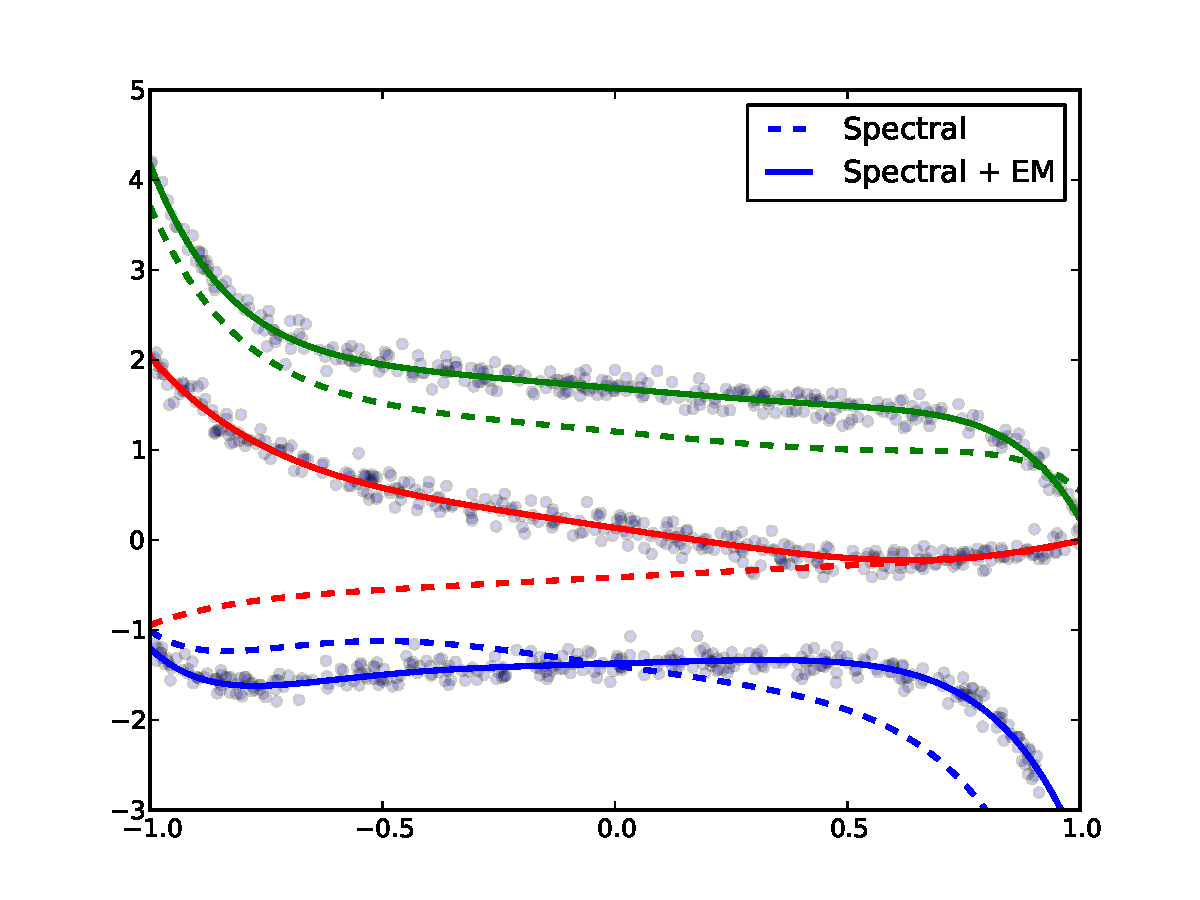
\includegraphics[width=0.50\textwidth]{figures/curves-vis/1-8-3-specm.pdf}}
    \hspace{-2em}
  \subfigure[EM]{
    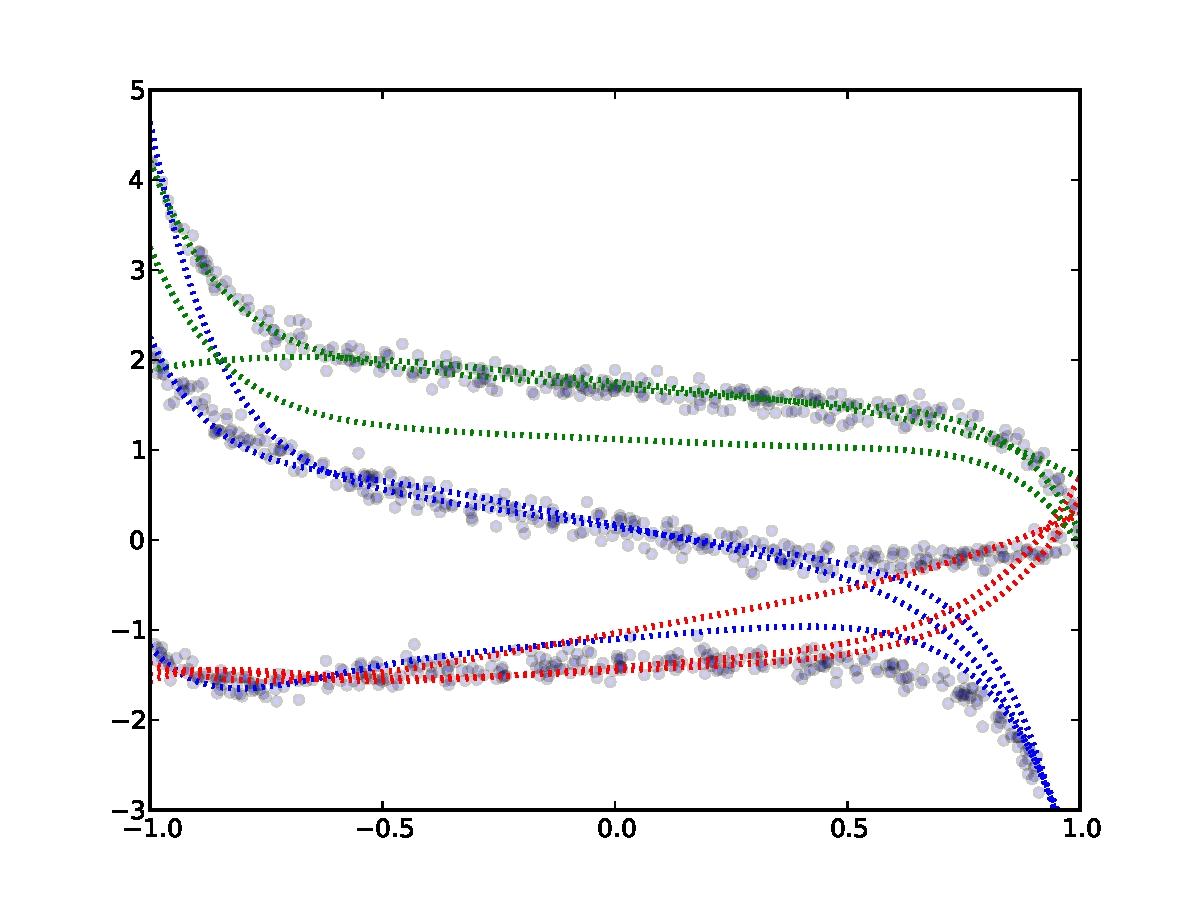
\includegraphics[width=0.50\textwidth]{figures/curves-vis/1-8-3-em.pdf}}
%  \subfigure[Spectral + EM]{
%    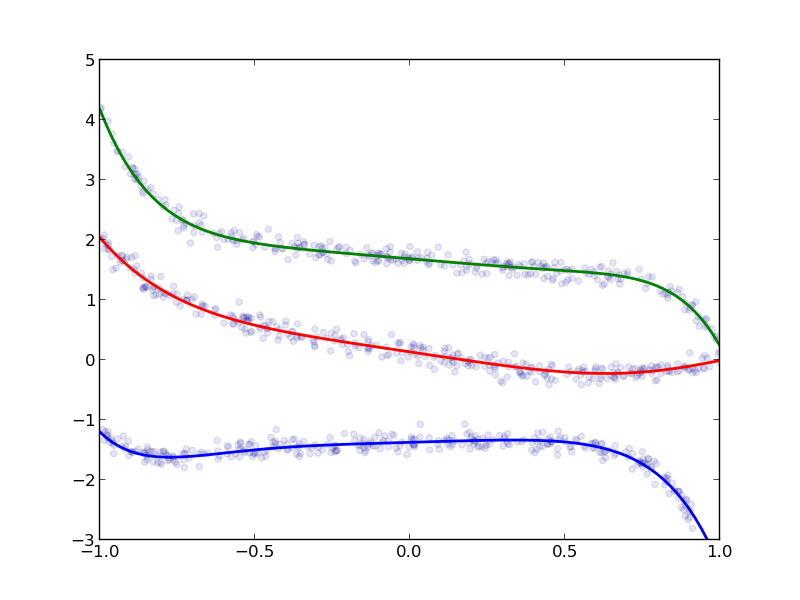
\includegraphics[width=0.34\textwidth]{figures/curves-vis/1-8-3-spem.png}}
  \caption{A comparison between Spectral Experts and EM. The dashed lines
  on the left denote the solution recovered by Spectral Experts. Whilst
  not a perfect fit, it provides an good initialization for EM to find
  the true global minima. The dotted lines on the right show different
  local optima found by EM on this example.}
  \label{fig:curves}
\end{figure*}

%Default values:
%$n = 10^6$
%$k = 5$

\begin{table*}[p]
\caption{Parameter Recovery Error $\|\theta^* - \hat \theta\|_F$ ($N = 500,000$).}
\label{tbl:parameter-recovery}
\vskip 0.15in
\begin{center}
\begin{small}
\begin{sc}

  \begin{tabular}{ r r r c c c }
\hline
\abovespace\belowspace
Variables ($b$) & Features ($D$) & Components ($K$) & Spectral & EM & Spectral + EM \\
\hline
\abovespace
%$\{1$, $ x_1$, $ x_1^4\}$ 
  1 & 4 & 2 & 1.52 $\pm$ 0.71 & 0.28 $\pm$ 0.82 & {\bf 0.13 $\pm$ 0.55} \\
%$\{1$, $ x_1$, $ x_2$, $ x_1^2 x_2^2\}$ 
  2 & 5 & 2 & 2.92 $\pm$ 1.10 & 0.00 $\pm$ 0.00 & {\bf 0.00 $\pm$ 0.00} \\
  2 & 5 & 3 & 3.76 $\pm$ 1.93 & 0.43 $\pm$ 1.07 & {\bf 0.23 $\pm$ 0.76} \\
%$\{1$, $ x_1$, $ x_2$, $ x_1 x_2^3$, $ x_1^2 x_2^2$, $ x_1^3 x_2 \}$ 
  2 & 6 & 2 & 4.52 $\pm$ 1.67 & 0.63 $\pm$ 1.29 & {\bf 0.18 $\pm$ 0.66} \\
\belowspace
  2 & 6 & 5 & 6.78 $\pm$ 2.18 & 2.29 $\pm$ 1.79 & {\bf 1.77 $\pm$ 1.89} \\

%  2 & 5 & 3 & 1.87 $\pm$ 1.20 & {\bf 0.33 $\pm$ 0.96} & 0.35 $\pm$ 1.23 \\
% 2 & 6 & 5 & 5.27 $\pm$ 2.32 & 1.80 $\pm$ 1.80 & {\bf 1.51 $\pm$ 1.77} \\
%$\{1$, $ x_1$, $ x_2$, $ x_1 x_2^3$, $ x_1^2 x_2^2$, $ x_1^3 x_2$, $ x_1^3 x_2^4$, $ x_1^4 x_2^3 \}$ 
% 2 & 8 & 7 & 8.42 $\pm$ 1.66 & 7.41 $\pm$ 2.99 & {\bf 7.31 $\pm$ 2.47} \\
%$\{1$, $ x_1$, $ x_2$, $ x_3$, $ x_1 x_2 x_3^2$, $ x_1 x_2^2 x_3$, $ x_1^2 x_2 x_3$, $ x_1^2 x_2^2$, $ x_1^2 x_3^2$, $ x_2^2 x_3^2$, $ x_3^2\}$
% 3 & 10 & 3 & 3.78 $\pm$ 0.90 & 0.67 $\pm$ 1.49 & {\bf 0.51 $\pm$ 1.12} \\
%$\{1$, $ x_1$, $ x_2$, $ x_3$, $ x_1 x_2 x_3^2$, $ x_1 x_2^2 x_3$, $ x_1^2 x_2 x_3$, $ x_1^2 x_2^2$, $ x_1^2 x_3^2$, $ x_2^2 x_3^2$, $ x_3^2\}$
% 3 & 10  & 7 & 9.97 $\pm$ 3.22 & 1.43 $\pm$ 1.97 & {\bf 1.42 $\pm$ 2.17} \\

\hline

\end{tabular}
\end{sc}
\end{small}
\end{center}
\vskip -0.1in
\end{table*}

% \todo{Dataset 2: $b = 30$, $p = 1$. I'm unclear as to what we can show
% on this sort of data set. EM works extremely well, and the spectral
% methods do not converge easily.}

\subsection{Results}

\tableref{tbl:parameter-recovery} presents the Fro\"ebenius norm of the
difference between true and estimated parameters for the model, averaged
over 20 different random instances for each feature set and 10 attempts
for each instance. The experiments were run using $N = 500,000$ samples.

One of the main reasons for the high variance is the variation across
random instances; some are easy for EM to find the global minima and
others more difficult. In general, while the spectral algorithm did not
recover parameters extremely well, it provided a good initialization for
EM.

\begin{figure}[th]
  \centering
  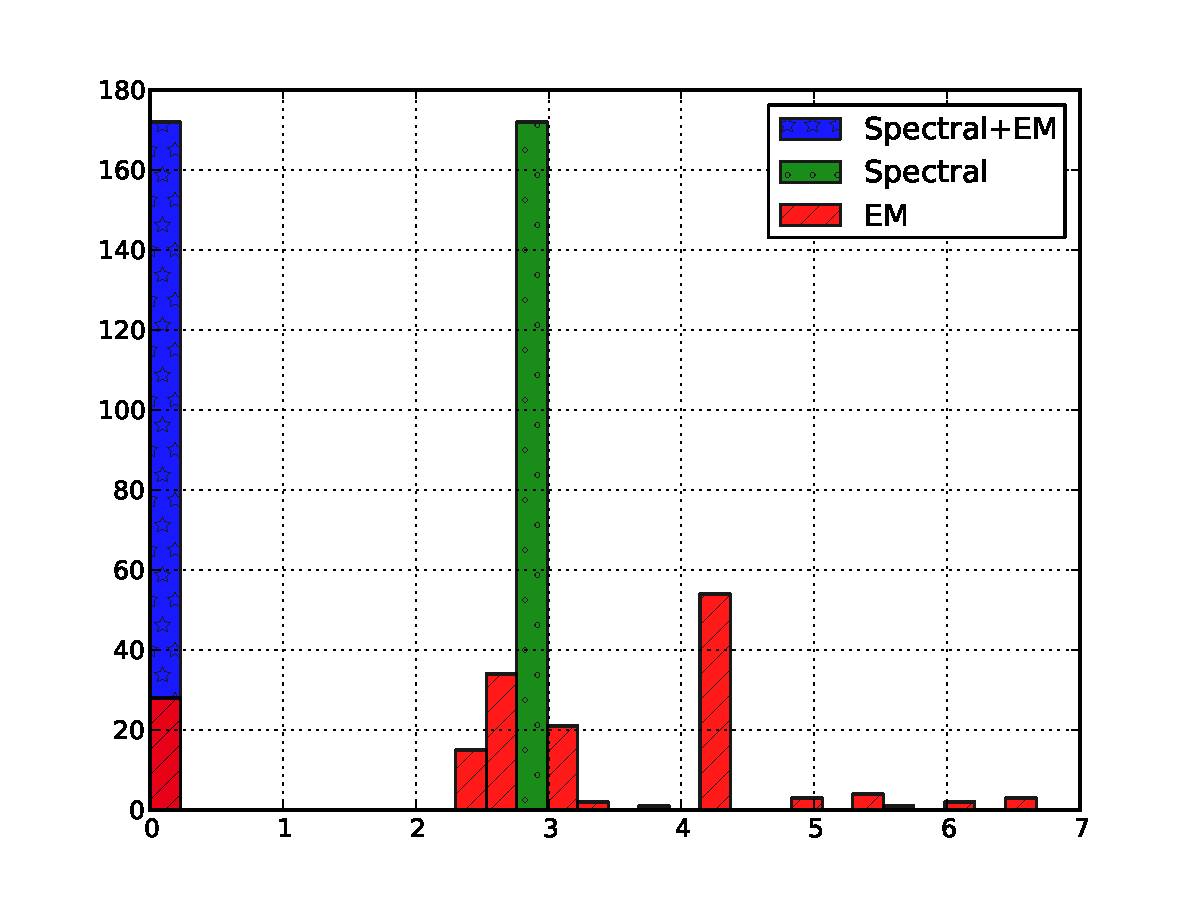
\includegraphics[width=0.50\textwidth]{figures/hist.pdf}
  \caption{Histogram over recovery errors between the three algorithms. $b = 1, d = 4, k = 3, N = 500,000$}
  \label{fig:hist}
\end{figure}

To study the stability of the solutions returned by the spectral method,
consider the histogram in \figureref{fig:hist}, which shows the recovery
errors of the algorithms over 170 attempts on a dataset with $b = 1, d = 4,
k = 3$. Typically, the spectral algorithm returned a stable solution.
When these parameters were close enough to the true parameters, we found
that EM almost always converged to the global optima. Randomly
initialized EM only finds the true parameters a little over 10\% of the
time and shows considerably higher variance. 

\paragraph{Effect of number of data points}

\begin{figure*}[p]
  \centering
  \subfigure[Well Data]{
    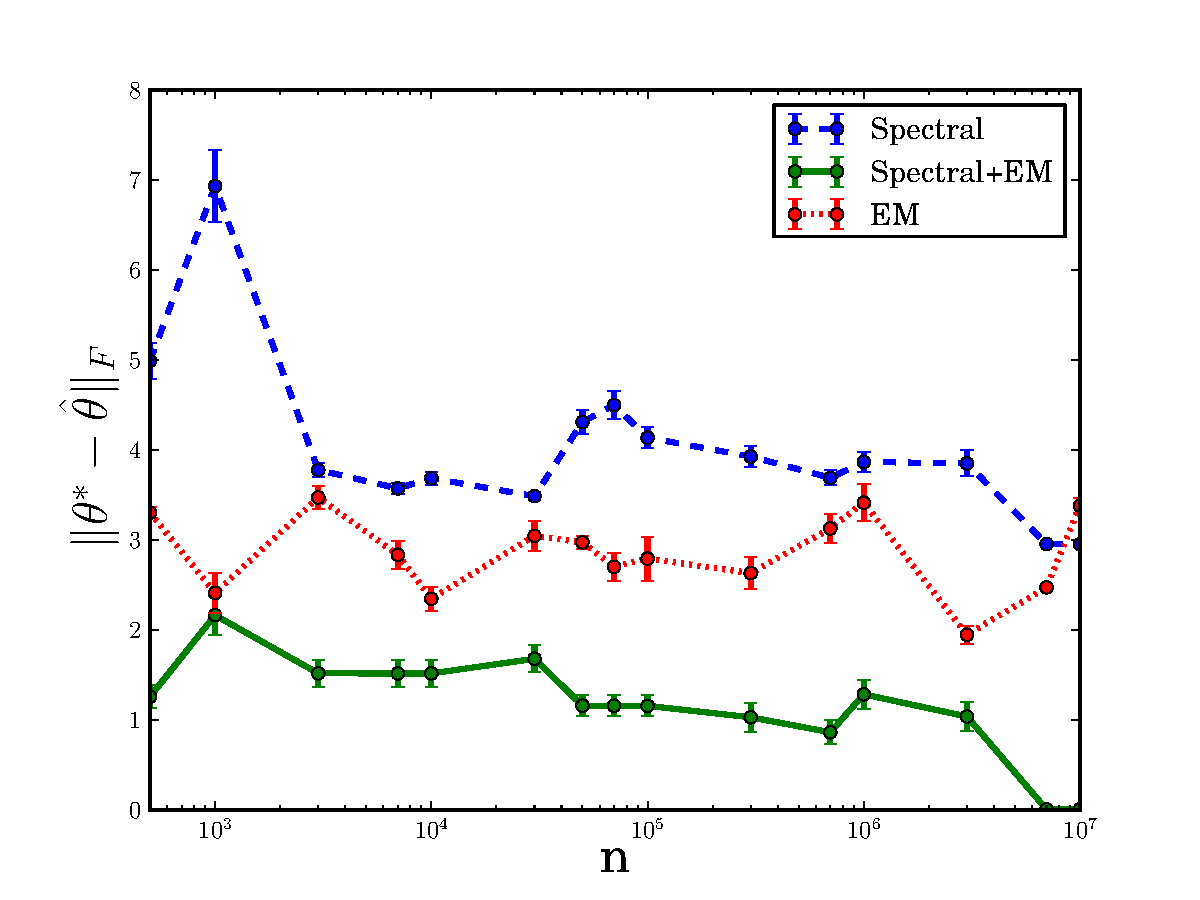
\includegraphics[width=0.50\textwidth]{figures/vs-n/1833-decay.pdf}
  }
    \hspace{-2em}
  \subfigure[Misspecified Data]{
    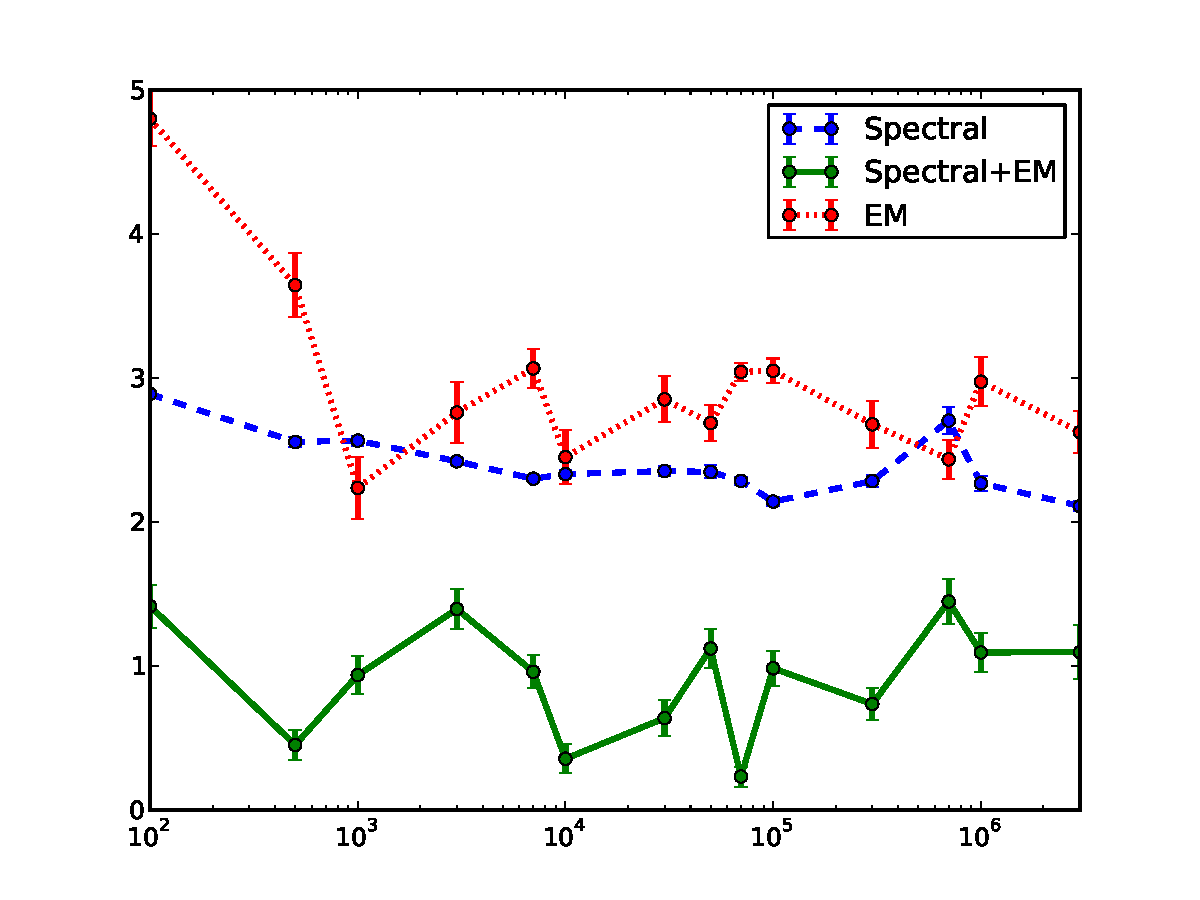
\includegraphics[width=0.50\textwidth]{figures/vs-n/1-8-3-3-rm.pdf}
  }
  \caption{Recovery error vs $n$  ($b = 1, d = 5, K = 3, N = 500,000$).}
  \label{fig:vs-n}
\end{figure*}

In \figureref{fig:vs-n}, we show how the recovery error varies as we get
more data. Each data point shows the mean error over 10 attempts, with
error bars. We note that the recovery performance of EM does not
particularly improve; this suggests that EM continues to get stuck in
a local optima. The spectral algorithm's error decays slowly, and as it
gets closer to zero, EM initialized at the spectral parameters finds the
true parameters more often as well. This behavior highlights the
trade-off between statistical and computational error. 

\paragraph{Misspecified Data}

\begin{table*}[t]
\caption{Parameter Recovery Error $\|\theta^* - \hat \theta\|_F$ with misspecified data ($N = 500,000$).}
\label{tbl:parameter-recovery-mis}
\vskip 0.15in
\begin{center}
\begin{small}
\begin{sc}

  \begin{tabular}{ r r r c c c }
\hline
\abovespace\belowspace
Variables ($b$) & Features ($d$) & Components ($K$) & Spectral & EM & Spectral + EM \\
\hline
\abovespace
 1 & 4 & 2 &  2.94 $\pm$ 1.52 & 0.29 $\pm$ 0.85 &  {\bf 0.22 $\pm$ 0.72} \\
\belowspace
 2 & 5 & 3 &  3.82 $\pm$ 2.00 & 0.44 $\pm$ 1.12 &  {\bf 0.35 $\pm$ 1.00} \\
 2 & 6 & 5 &  9.89 $\pm$ 4.46 & {\bf 2.53 $\pm$ 1.77} &  2.69 $\pm$ 1.83 \\
 2 & 8 & 7 & 23.07 $\pm$ 7.10 & 9.62 $\pm$ 1.03 &  {\bf 8.16 $\pm$ 2.31}  \\
\hline

\end{tabular}
\end{sc}
\end{small}
\end{center}
\vskip -0.1in
\end{table*}

To evaluate how robust the algorithm was to model mis-specification, we
removed large contiguous sections from $x \in [-0.5,-0.25] \cup
[0.25,0.5]$ and ran the algorithms again.
\tableref{tbl:parameter-recovery-mis} reports recovery errors in this
scenario. The error in the estimates grows larger for higher $d$.


\section{Conclusion}
\label{sec:conclusion}



\appendix
\section{Regression}

Let us review the regression problem set up in \cite[Section
3]{ChagantyLiang2013}. We assume we are given data $(x_i,y_i) \in \sD_p$
generated by the following process,
\begin{align}
  y_i &= \innerp{M_p}{x_i\tp{p}} + \eta_p(x_i),
\end{align}
where $M_p = \sum_{h=1}^k \pi_h \beta_h\tp{p}$, the p-th order moments
of $\beta_h$ and $\eta_p(x)$ is zero mean noise. In particular, for $p \in \{1,2,3\}$,
we showed that $\eta_p(x)$ were defined to be,
\begin{align}
  \eta_1(x) &= \innerp{\beta_h - M_1}{x} + \epsilon \label{eqn:eta1} \\
  \eta_2(x) &= \innerp{\beta_h\tp{2} - M_2}{x\tp{2}} + 2 \epsilon \innerp{\beta_h}{x} + (\epsilon^2 - \E[\epsilon^2]) \label{eqn:eta2}\\
  \eta_3(x) &= \innerp{\beta_h\tp{3} - M_3}{x\tp{3}}
        + 3 \epsilon \innerp{\beta_h\tp{2}}{x\tp{2}} 
        + 3(\epsilon^2 \innerp{\beta_h}{x} - \E[\epsilon^2] \innerp{M_1}{x})
        + (\epsilon^3 - \E[\epsilon^3]). \label{eqn:eta3}
\end{align}
We assume that $\|x_i\| \le R$, $\| \beta_h \| \le L$ and $|\epsilon| \le S$.

We then defined the observation operator $\opX_p(M_p) : \Re^{d\tp{p}} \to \Re^{n}$,
\begin{align}
\opX_p(M_p; \sD_p)_i &\eqdef \innerp{M_p}{x\tp{p}_i}, & (x_i, y_i) \in \sD_p,
\end{align}
which let us succinctly represent the low-rank regression problem as follows,
\begin{align}
  \min_{M_p \in \Re^{d\tp{p}}} \frac{1}{2n} \| y - \opX_p(M_p; \sD_p) \|^2_2 + \lambda_p \|M_p\|_*.
\end{align}

Let us also recall the adjoint of the observation operator, $\opX_p^* : \Re^{n} \to \Re^{d^p}$,
\begin{align}
  \opX_p^*(\eta_p; \sD_p) &= \sum_{x \in \sD_p} \eta_p(x) x\tp{p},
\end{align}
where we have used $\eta_p$ to represent the vector $\left[\eta_p(x)\right]_{x \in \sD_p}$. 

\citet{Tomioka2011} showed that error in the estimated $\hat M_p$ can be
bounded as follows;

\begin{lemma}[\citet{Tomioka2011}, Theorem 1]
\label{lem:lowRank}
Suppose there exists a restricted strong convexity constant $\kappa(\opX_p)$ such that
$$\frac{1}{2n} \| \opX_p( \Delta )\|_2^2 \ge \kappa(\opX_p) \|\Delta\|^2_F \quad \text{and} \quad
\lambda_n \ge \frac{\|\opX_p^*(\eta_p)\|_\op}{n}.$$
Then the error of $\hat M_p$ is bounded as follows:
$\| \hat M_p - M_p^* \|_F \le \frac{\lambda_n \sqrt{k}}{\kappa(\opX_p)}$.
\end{lemma}

In this section, we will derive an upper bound on $\kappa(\opX_p)$ and
a lower bound on $\frac{1}{n} \| \opX_p^*(\eta_p) \|_\op$.

\begin{lemma}[Lower bound on restricted strong convexity]
\label{lem:lowRankLower}
Let $\Sigma_p \eqdef \E[\cvec(x\tp{p})\tp{2}]$.
If $$n \ge \frac{16 (p!)^2 R^{4p}}{\sigmamin(\Sigma_p)^2} \left(1 + \sqrt{\frac{\log(1/\delta)}{2}}\right)^2,$$
then, with probability at least $1-\delta$,
$$\kappa(\opX_p) \ge \frac{\sigmamin(\Sigma_p)}{2}.$$
\end{lemma}

\begin{proof}
  Recall the definition of $\kappa(\opX_p)$, 
  $$\frac{1}{n} \|\opX_p(\Delta)\|_2^2 \ge \kappa(\opX_p) \|\Delta\|^2_F.$$
Expanding the definition of the observation operator:
$$\frac{1}{n} \|\opX_p(\Delta)\|_2^2 = \frac{1}{n} \sum_{(x,y) \in \sD_p} \innerp{\Delta}{x\tp{p}}^2.$$
Unfolding the tensors, letting $\hat\Sigma_p \eqdef \frac{1}{n}
\sum_{(x,y) \in \sD_p} \cvec(x\tp{p})\tp{2}$, $\frac{1}{n}
\|\opX_p(\Delta)\|_2^2 = \trace(\cvec(\Delta)\tp{2} \hat\Sigma_p)$. 
We recall that each element of $\cvec(\Delta)$ aggregates elements with
permuted indices, so $\|\vvec(\Delta)\|_2 \le \|\cvec(\Delta)\|_2 \le p!
\|\vvec(\Delta)\|_2$. Then, we have 
\begin{align}
\frac{1}{n} \|\opX_p(\Delta)\|_2^2 
  &= \trace(\cvec(\Delta)\tp{2} \hat\Sigma_p) \\
  &\ge \sigmamin(\hat\Sigma_p) \|\Delta\|_F^2 .
\end{align}
By Weyl's theorem, $$\sigmamin(\hat\Sigma_p) \ge
\sigmamin(\Sigma_p) - \|\hat\Sigma_p - \Sigma_p\|_\Lop.$$
Since $\|\hat\Sigma_p - \Sigma_p\|_\Lop \le \|\hat\Sigma_p - \Sigma_p\|_{F}$,
it suffices to show that the empirical covariance concentrates in Frobenius norm.
Applying \reflem{conc-norms}, with
probability at least $1 - \delta$, $$\| \hat\Sigma_p - \Sigma_p \|_F
\le \frac{2 \|\Sigma_p\|_F}{\sqrt n} \left( 1 + \sqrt{\frac{\log(1/\delta)}{2}} \right).$$
Now we seek to control $\|\Sigma_p\|_F$.
Since $\|x\|_2 \le R$, we can use the
bound $$\| \Sigma_p \|_F \le p! \| \vvec(x\tp{p})\tp{2} \|_F \le p! R^{2p}.$$

Finally, $\|\hat\Sigma_p - \Sigma_p\|_\op \le \sigmamin(\Sigma_p)/2$ with probability at least $1 - \delta$ if,
$$n \ge \frac{16 (p!)^2 R^{4p}}{\sigmamin(\Sigma_p)^2} \left(1 + \sqrt{\frac{\log(1/\delta)}{2}}\right)^2.$$

%To do this, we first apply Hoeffding's inequality elementwise.
%Since $\|x\|_2 \le R$, we have that for each element $(i,j)$,
%$|(\hat\Sigma_p)_{ij} - (\Sigma_p)_{ij}| = O(R^{2p}\sqrt{\frac{\log (1/\delta)}{n}})$.
%Applying the union bound over the $d^{2p}$ elements of $\hat\Sigma_p - \Sigma_p$,
%we have that the max norm is bounded:
%$\|\hat\Sigma_p - \Sigma_p\|_\text{\rm max} = O(R^{2p} \sqrt{\frac{p \log(d) \log (1/\delta)}{n}})$.
%The max norm times $d^p$ upper bounds the Frobenius norm, which upper bounds the operator norm, so we have that
%$\|\hat\Sigma_p - \Sigma_p\|_\text{\rm op} = O(d^p R^{2p} \sqrt{\frac{p \log(d) \log (1/\delta)}{n}})$.
%Using the fact that $\sigmamin(\hat\Sigma_p) \ge \sigmamin(\Sigma_p) - \|\hat\Sigma_p - \Sigma_p\|_\text{\rm op}$
%yields the result.
\end{proof}

\begin{lemma}[Upper bound on adjoint operator]
\label{lem:lowRankUpper}
With probability at least $1-\delta$, the following holds,
\begin{align*}
  \frac{1}{n} \|\opX_1^*(\eta_1)\|_\op
      &\le \frac{2R (2LR + S)}{\sqrt{n}} \left( 1 + \sqrt{\frac{\log(3/\delta)}{2}} \right) \\
  \frac{1}{n}  \|\opX_2^*(\eta_2)\|_\op 
      &\le \frac{(4L^2 R^2 + 2 S L R + 4S^2)R^2}{\sqrt{n}} \left( 1 + \sqrt{\frac{\log(3/\delta)}{2}} \right) \\
  \frac{1}{n} \|\opX_3^*(\eta_3)\|_\op 
      &\le \frac{(8L^3 R^3 + 3 L^2 R^2 S + 6 L R S^2 + 2S^3) R^3}{\sqrt{n}} \left( 1 + \sqrt{\frac{\log(6/\delta)}{2}} \right) \\
  &\quad + 3 R^4 S^2 \left(\frac{4R(2LR+S)}{\sigmamin(\Sigma_1) \sqrt{n}} \left(1 + \sqrt{\frac{\log(6/\delta)}{2}} \right) \right).
\end{align*}
\end{lemma}

It follows that, with probability at least $1-\delta$,
\begin{align*}
  \frac{1}{n} \|\opX_p^*(\eta_p)\|_\op
  &= O\left( L^p S^p R^{2p} \sigmamin(\Sigma_1)^{-1} \sqrt{\frac{\log(1/\delta)}{n}} \right),
\end{align*}
for each $p \in \{1,2,3\}$.

\begin{proof}
Let $\hat\E_p[f(x,\epsilon,h)]$ denote the empirical expectation over
the examples in dataset $\sD_p$ (recall the $\sD_p$'s are independent to
simplify the analysis).  By definition,
$$\frac1n \|\opX_p^*(\eta_p)\|_\op = \left\| \hat\E_p[\eta_p(x) x\tp{p}] \right\|_\op $$
for $p \in \{1,2,3\}$. To proceed, we will bound each $\eta_p(x)$, defined in \refeqn{eta1},
\refeqn{eta2} and \refeqn{eta3} and use \reflem{conc-norms} to bound $\|
\hat\E_p[\eta_p(x) x\tp{p}] \|_F$. The Frobenius norm to bounds the
operator norm, completing the proof.

%composed of several zero-mean random variables, and
%since $\|A + B\|_\op \le \|A\|_\op + \|B\|_\op$, it suffices to consider
%each term in turn. 

\paragraph{Bounding $\eta_p(x)$.}
Using the assumptions that $\|\beta_h\|_2 \le L$, $\|x\|_2 \le R$ and
$|\epsilon| \le S$, it is easy to bound each $\eta_p(x)$,
\begin{align*}
  \eta_1(x) &= \innerp{\beta_h - M_1}{x} + \epsilon \\
            &\le \|\beta_h - M_1\|_2 \|x\|_2 + |\epsilon| \\
            &\le 2LR + S \\
  \eta_2(x) 
    &= \innerp{\beta_h\tp{2} - M_2}{x\tp{2}} + 2 \epsilon \innerp{\beta_h}{x} + (\epsilon^2 - \E[\epsilon^2]) \\
    &\le \|\beta_h\tp{2} - M_2\|_F \|x\tp{2}\|_F + 2 |\epsilon| \|\beta_h\|_2\|x\|_2 + |\epsilon^2 - \E[\epsilon^2]| \\
    &\le (2L)^2 R^2 + 2 S L R + (2S)^2 \\
  \eta_3(x) &= \innerp{\beta_h\tp{3} - M_3}{x\tp{3}}
        + 3 \epsilon \innerp{\beta_h\tp{2}}{x\tp{2}} \\
        &\quad + 3\left(\epsilon^2 \innerp{\beta_h}{x} - \E[\epsilon^2] \innerp{\hat M_1}{x}\right)
        + (\epsilon^3 - \E[\epsilon^3]) \\
  &\le \|\beta_h\tp{3} - M_3\|_F\|x\tp{3}\|_F
        + 3 |\epsilon| \|\beta_h\tp{2}\|_F \|x\tp{2}\|_F  \\
        &\quad + 3 \left( |\epsilon^2|~\|\beta_h\|_F\|x\|_F + \left|\E[\epsilon^2]\right|~\|\hat M_1\|_2\|x\|_2 \right)
        + |\epsilon^3| + \left| \E[\epsilon^3] \right| \\
  &\le (2L)^3 R^3 + 3 S L^2 R^2 + 3 ( S^2 L R + S^2 L R ) + 2S^3.
\end{align*}
We have used inequality $\|M_1 - \beta_h\|_2 \le 2L$ above. 

\paragraph{Bounding $\left\| \hat\E[\eta_p(x)x\tp{p}] \right\|_F$.}
We may now apply the above bounds on $\eta_p(x)$ to bound $\|\eta_p(x) x\tp{p}\|_F$, using the fact that $\|c X\|_F \le c\|X\|_F$.
By \reflem{conc-norms}, each of the following holds with probability at least $1-\delta_1$,
\begin{align*}
    \left\|\hat\E_1[\eta_1(x) x] \right\|_2
    &\le \frac{2R (2LR + S)}{\sqrt{n}} \left( 1 + \sqrt{\frac{\log(1/\delta_1)}{2}} \right) \\
  \left\|\hat\E_2[\eta_2(x) x\tp{2}] \right\|_F
      &\le \frac{(4L^2 R^2 + 2 S L R + 4S^2)R^2}{\sqrt{n}} \left( 1 + \sqrt{\frac{\log(1/\delta_2)}{2}} \right) \\
  \left\|\hat\E_3[\eta_3(x) x\tp{3}] - \E[\eta_3(x) x\tp{3} \mid x] \right\|_F
      &\le \frac{(8L^3 R^3 + 3 L^2 R^2 S + 6 L R S^2 + 2S^3) R^3}{\sqrt{n}} \left( 1 + \sqrt{\frac{\log(1/\delta_3)}{2}} \right).
\end{align*}

Recall that $\eta_3(x)$ does not have zero mean, so we must bound the bias:
\begin{align*}
  \| \E[\eta_3(x) x\tp{3} \mid x] \|_F &= \|3 \E[\epsilon^2] \innerp{M_1 - \hat M_1}{x} x\tp{3} \|_F \\
    &\le 3 \E[\epsilon^2] \|M_1 - \hat M_1\|_2 \|x\|_2 \|x\tp{3}\|_F.
\end{align*}
Note that in all of this, both $\hat M_1$ and $M_1$ are treated as
constants. Further, by applying \reflem{lowRank}, we have a bound on $\|M_1 - \hat
M_1\|_2$. So, with probability at least $1 - \delta_3$,
\begin{align*}
  \| \E[\eta_3(x) x\tp{3} \mid x] \|_F
  &\le 3 R^4 S^2 \left(\frac{4R(2LR+S)}{\sigmamin(\Sigma_1) \sqrt{n}} \left(1 + \sqrt{\frac{\log(1/\delta_3)}{2}} \right) \right).
\end{align*}

% {%
% \begin{align*}
% %   \| \hat\E_1[ \eta_1(x) x ] \|_\Lop &\le 
% %             \underbrace{ \|\hat\E_1[\innerp{M_1 - \beta_h}{x} x]\|_\op  }_{ O( L R^2     \sqrt{\frac{\log(1/\delta_1)}{n}} ) } +
% %             \underbrace{ \|\hat\E_1[\epsilon x]\|_\op                   }_{ O( R S  \sqrt{\frac{\log(1/\delta_1)}{n}} ) } \\
%   %  &= O( S L R^2 \sqrt{\frac{\log(1/\delta_1)}{n}} ) \\
%     \| \hat\E_2[ \eta_2(x) x\tp{2} ] \|_\Lop &\le 
%             \underbrace{ \|\hat\E_2[\innerp{\beta_h\tp{2} - M_2}{x\tp{2}} x\tp{2}]\|_\op }_{ O( L^2 R^4      \sqrt{\frac{\log(1/\delta_1)}{n}} ) } \\
%    &\quad + \underbrace{ \|\hat\E_2[2 \epsilon \innerp{\beta_h}{x} x\tp{2}]\|_\op        }_{ O( S L R^3 \sqrt{\frac{\log(1/\delta_1)}{n}} ) } 
%           + \underbrace{ \|\hat\E_2[(\epsilon^2 - S^2) x\tp{2}]\|_\op               }_{ O( S^2 R^2 \sqrt{\frac{\log(1/\delta_1)}{n}} ) } \\
%   %&= O( S^2 L^2 R^4 \sqrt{\frac{\log^2(1/\delta_1)}{n}} ) \\
%   \| \hat\E_3[ \eta_3(x) x\tp{3} ] \|_\Lop &\le 
%             \underbrace{ \|\hat\E_3[\innerp{\beta_h\tp{3} - M_3}{x\tp{3}}                      x\tp{3}]\|_\op }_{O( L^3 R^6        \sqrt{\frac{\log(1/\delta_1)}{n}} ) } \\
%    &\quad + \underbrace{ \|\hat\E_3[3 \epsilon \innerp{\beta_h\tp{2}}{x\tp{2}}                 x\tp{3}]\|_\op }_{O( S L^2 R^5 \sqrt{\frac{\log(1/\delta_1)}{n}} ) } 
%           + \underbrace{ \|\hat\E_3[\epsilon^3                                                 x\tp{3}]\|_\op }_{O( S^3 R^3   \sqrt{\frac{\log (1/\delta_1)}{n}} ) } \\
%    &\quad + \underbrace{ \|\hat\E_3[3(\epsilon^2 \innerp{\beta_h}{x} -S^2 \innerp{\hat M_1}{x}) x\tp{3}]\|_\op }_{O( (S^2 L R^4 + S^2 R^4) \sqrt{\frac{\log(1/\delta_1)}{n}} ) } \\
%   %&= O( S^3 L^3 R^6 \sqrt{\frac{\log^3(1/\delta_1)}{n}} ).
% \end{align*}
% }
% There are two additional considerations when bounding the terms in $\eta_3$.
% First, to bound $\hat\E_3[\epsilon^3]$, we use Lemma 19 of \cite{hsu13spherical}.
% Second, there is an additional bias since the estimator uses $\hat M_1$ instead of $M_1$; this bias is small by the previous bound (and is constructed on an independent dataset, $\sD_1$).
% Therefore, we incur another $O(S^2 \cdot R^4 \sqrt{\frac{\log(1/\delta_1)}{n}})$.
%We can handle the other terms using conventional means, the details of which can be found in \appendixref{sec:proofs}.
%Note that we are bounding quantities fairly crudely for the sake of simplicity.

Finally, taking $\delta_1 = \delta/3, \delta_2 = \delta/3, \delta_3
= \delta/6$, and taking the union bound over the bounds for $p \in
\{1,2,3\}$, we get our result.
\end{proof}

%%%%%%%%%%%%

\section{Tensor Decomposition}

Once we have estimated the moments from the data through regression, we apply the robust tensor eigen-decomposition algorithm to recover the parameters, $\beta_h$ and $\pi$. However, the algorithm is guaranteed to work only for symmetric matrices with (nearly) orthogonal eigenvectors, so as a first step, we will need to whiten the third-order moment tensor using the second moments. Once we get the eigenvalues and eigenvectors from this orthogonal tensor, we have to undo the transformation by applying an un-whitening step. In this section, we present error bounds for each step, and combine them to prove the following lemma,
\begin{lemma}[Tensor Decomposition with Whitening]
  \label{lem:tensorPower} 
  Let $M_3 = \sum_{h=1}^{k} \pi_h \beta_h\tp{3}$.
  Let $\|\hat M_2 - M_2\|_\op$ and
  $\|\hat M_3 - M_3\|_\op$ both be less than
  \begin{align*}
    \frac{3\sigma_k(M_2)^{3/2}}{10 k \pi_{\max}^{5/2}
    \left(24 \frac{\| {M_3} \|_\op}{\sigma_k(M_2)} + 2\sqrt{2} \right)}~ \epsilon,
  \end{align*}
  and,
\begin{align*}
  \frac{\sigma_k(M_2)}
    {\|M_2\|_\op^{1/2} \left(
    4\sqrt{3/2} + 8 k \pi_{\max} 
    \sigma_k(M_2)^{-1/2}
    \left(24 \frac{\| {M_3} \|_\op}{\sigma_k(M_2)} + 2\sqrt{2} \right) \right) }~ \epsilon,
\end{align*}
for some $\epsilon$ such that 
\begin{align}
  \epsilon &\le 
    \min\Bigg\{
      \Bigg( 4\sqrt{3/2} \|M_2\|_\op^{1/2} \sigma_k(M_2)^{-1} \aerr{M_2} \\
     &\quad + 8 \|M_2\|_\op^{1/2} k \pi_{\max} \sigma_k(M_2)^{-3/2}
        \left(24 \frac{\| {M_3} \|_\op}{\sigma_k(M_2)} + 2\sqrt{2} \right) \Bigg) \frac{\sigma_k(M_2)}{2}, \\
  &\quad \left( \frac{2 \pi_{\max}^{3/2}}{3} 5 k \pi_{\max} 
    \sigma_k(M_2)^{-3/2}
    \left(24 \frac{\| {M_3} \|_\op}{\sigma_k(M_2)} + 2\sqrt{2} \right)  \right) \frac{\sigma_k(M_2)}{2}, \\
      &\quad \frac{1}{2\sqrt{\pi_{\max}}} \\
   &\quad \Bigg\}.
\end{align}

  Then, there exists a permutation of indices such that  the parameter
  estimates found in step 2 of \citet[Algorithm 1]{ChagantyLiang2013}
  satisfy the following with probability at least $1 - \delta$,
  \begin{align*}
  \|\hat \pi - \pi \|_{\infty} &\le \epsilon \\
  \|\hat \beta_h - \beta_h\|_2 &\le \epsilon.
  \end{align*}
  for all $h \in [k]$.
\end{lemma}

\begin{proof}
We will use the general notation, $\aerr{X} \eqdef \|\hat X - X\|_\Lop$
to represent the error of the estimate, $\hat X$, of $X$ in the operator
norm. 
\paragraph{Step 1: Whitening}
Let $W$ and $\hat W$ be the whitening matrices for $M_2$ and $\hat M_2$
respectively. Also define $\Winv$ and $\Whinv$ to be their
pseudo-inverses.

We will first show that the whitened tensors $T = M_3(W,W,W)$ and $\hat
T = \hat M_3(\hat W, \hat W, \hat W)$ are symmetric with orthogonal
eigenvectors. Recall that $M_2 = \sum_h \pi_h \beta_h\tp{2}$, and thus
$W \beta_h = \frac{v_h}{\sqrt{\pi_h}}$, where $v_h$ form an orthonormal
basis. Applying the whitening transform to $M_3$, we get, 
\begin{align}
  M_3 &= \sum_h \pi_h \beta_h\tp{3} \\
  M_3(W,W,W) &= \sum_h \pi_h (W\beta_h)\tp{3} \\
  &= \sum_h \frac{1}{\sqrt{\pi_h}} v_h\tp{3}.
\end{align}
Consequently, $T$ has orthogonal eigenvectors, with eigenvalues $1/\sqrt{\pi_h}$.

Let us now study how far $\hat T$ differs from $T$, in terms of the
errors of $M_2$ and $M_3$. To do so, we use the triangle inequality to
break the difference into a number of simple terms,
\begin{align*}
  \aerr{T} &= \|M_3(W,W,W) - \hat M_3(\hat W,\hat W, \hat W)\|_\op \\
           &\le 
           \| {M_3}(W,W,W) - {M_3}(W,W,\hat W) \|_\op
           + \| {M_3}(W,W,\hat W) - {M_3}(W, \hat W, \hat W)\|_\op \\
           &\quad 
           + \|{M_3}(W,\hat W,\hat W) - {M_3}(\hat W, \hat W, \hat W)\|_\op 
           + \|{M_3}(\hat W,\hat W,\hat W) - - \hat {M_3}(\hat W,\hat W, \hat W)\|_\op \\
           &\le
           \| {M_3} \|_\op \|W\|^2_\op \aerr{W} +
            \| {M_3} \|_\op \|\hat W\|_\op \|W\|_\op \aerr{W} +
            \| {M_3} \|_\op \|\hat W\|^2_\op \aerr{W} +
            \aerr{M_3} \|\hat W\|^3_\op  \\
           &\le
           \| {M_3} \|_\op (\|W\|^2_\op + \|\hat W\|_\op \|W\|_\op + \|\hat W\|^2_\op) \aerr{W} +
            \aerr{M_3} \|\hat W\|^3_\op 
\end{align*}
We can relate $\|\hat W\|$ and $\aerr{W}$ to $\aerr{M_2}$ using using
\refprop{white}. The conditions on $\aerr{M_2}$ imply that $\aerr{M_2}
< \sigma_k(M_2)/2$, giving us,
\begin{align*}
  \|\hat W\|_\op &\le \sqrt{2} \sigma_k(M_2)^{-1/2} \\
  \aerr{W} &\le 4 \sigma_k(M_2)^{-3/2} \aerr{M_2}.
\end{align*}
Thus,
\begin{align*}
  \aerr{T} &\le 
  6 \| {M_3} \|_\op \|W\|^2_\op (4 \sigma_k(M_2)^{-3/2}) \aerr{M_2} +
  \aerr{M_3} 2\sqrt{2} \|W\|^3_\op \\
  &\le 
  24 \| {M_3} \|_\op \sigma_k(M_2)^{-5/2} \aerr{M_2} +
  2\sqrt{2} \sigma_k(M_2)^{-3/2} \aerr{M_3} \\
  &\le 
    \sigma_k(M_2)^{-3/2}
      \left(24 \frac{\| {M_3} \|_\op}{\sigma_k(M_2)} + 2\sqrt{2} \right)
      \max\{ \aerr{M_2}, \aerr{M_3} \}.
\end{align*}

\paragraph{Step 2: Decomposition}

We have constructed $T$ to be a symmetric tensor with orthogonal
eigenvectors. We can now apply the results of \citet[Theorem
5.1]{AnandkumarGeHsu2012} to bound the error in the eigenvalues,
$\lambda_W$, and eigenvectors, $\omega$, returned by the robust tensor
power method;
\newcommand{\lW}{\lambda_W}
\newcommand{\lhW}{{\hat\lambda}_W}
\newcommand{\mW}{\omega}
\newcommand{\mhW}{{\hat\omega}}
\begin{align}
  \|\lW - \lhW \|_{\infty} 
  &\le \frac{5 k \aerr{T}}{(\lW)_{\min}} \\
\|\mW_h -\mhW_h \|_2 
&\le \frac{8 k \aerr{T}}{(\lW)_{\min}^2},
\end{align}
for all $h \in [k]$, where $(\lW)_{min}$ is the smallest
eigenvalue of $T$. 

\paragraph{Step 3: Unwhitening}

Finally, we need to invert the whitening transformation to recover $\pi$ and
$\beta_h$ from $\lW$ and $\mW_h$. Let us complete the proof by
studying how this inversion relates the error in $\pi$ and $\beta$ to
the error in $\lW$ and $\mW$.

First, we will bound the error in the $\beta$s,
\begin{align*}
  \|\hat \beta_h - \beta_h\|_2
  &= \| \Whinv \mhW - \Winv \mW \|_2 \\
  &\le \aerr{\Winv} \|\mhW_h\|_2 + \|\Winv\|_2 \|\mhW_h - \mW_h \|_2. \comment{Triangle inequality}
\end{align*}

Once more, we can apply the results of \refprop{white}, with the assumptions on $\aerr{M_2}$, to get, 
\begin{align*}
  \|\Whinv\|_\op &\le \sqrt{3/2} \|M_2\|_\op^{1/2} \\
  \aerr{\Winv} &\le 4\sqrt{3/2} \|M_2\|_\op^{1/2} \sigma_k(M_2)^{-1} \aerr{M_2}.
\end{align*}

Thus,
\begin{align*}
  \|\hat \beta_h - \beta_h\|_2
  &\le 4\sqrt{3/2} \|M_2\|_\op^{1/2} \sigma_k(M_2)^{-1} \aerr{M_2} 
    + 8 \|M_2\|_\op^{1/2} \frac{k \aerr{T}}{(\lW)_{min}^2} \\
    &\le 4\sqrt{3/2} \|M_2\|_\op^{1/2} \sigma_k(M_2)^{-1} \aerr{M_2} \\
  &\quad + 8 \|M_2\|_\op^{1/2} k \pi_{\max} 
    \sigma_k(M_2)^{-3/2}
      \left(24 \frac{\| {M_3} \|_\op}{\sigma_k(M_2)} + 2\sqrt{2} \right)
      \max\{\aerr{M_2}, \aerr{M_3}\}.
\end{align*}

Next, let us bound the error in $\pi$,
\begin{align*}
  |\hat \pi_h - \pi_h |
  &= \left| \frac{1}{(\lW)_h^2} - \frac{1}{(\lhW)_h^2} \right| \\
  &= \left| \frac{\left( (\lW)_h + (\lhW)_h \right) \left( (\lW)_h - (\lhW)_h \right)}
  {(\lW)_h^2(\lhW)_h^2} \right| \\
  &\le \frac{( 2(\lW)_h - \|\lW - \lhW\|_{\infty} )}{(\lW)_h^2 \left( (\lW)_h + \|\lW - \lhW\|_{\infty} \right)^2} \|\lW - \lhW\|_{\infty}.
\end{align*}
Recall that $(\lW)_h = \pi_h^{-1/2}$, so the
assumptions that $\epsilon$ imply that $\|\lW - \lhW \|_{\infty} \le
(\lW)_{\min}/2$. This allows us to simplify the above expression as
follows,
\begin{align*}
  |\hat \pi_h - \pi_h |
  &\le \frac{(3/2)(\lW)_h}{(3/2)^2 (\lW)_h^4}
  \|\lW - \lhW\|_{\infty} \\
  &\le \frac{2}{3(\lW)_h^3} \frac{5 k \aerr{T}}{(\lW)_{\min}^2} \\
  &\le \frac{2 \pi_{\max}^{3/2}}{3} 5 k \pi_{\max} 
    \sigma_k(M_2)^{-3/2}
    \left(24 \frac{\| {M_3} \|_\op}{\sigma_k(M_2)} + 2\sqrt{2} \right) \max\{\aerr{M_2}, \aerr{M_3}\}.
\end{align*}

We complete the proof by requiring that the bounds $\aerr{M_2}$ and
$\aerr{M_3}$ imply that $\|\hat \pi - \pi \|_{\infty} \le \epsilon$ and
$\|\hat \beta_h - \beta_h\|_2 \le \epsilon$, i.e.
\begin{align*}
  \max\{\aerr{M_2}, \aerr{M_3}\} &\le 
  \frac{3\sigma_k(M_2)^{3/2}}{10 k \pi_{\max}^{5/2}
  \left(24 \frac{\| {M_3} \|_\op}{\sigma_k(M_2)} + 2\sqrt{2} \right)}~ \epsilon,
\end{align*}
as well as,
\begin{align*}
  \max\{\aerr{M_2}, \aerr{M_3}\} 
  &\le 
  \frac{\sigma_k(M_2)}
    {\|M_2\|_\op^{1/2} \left(
    4\sqrt{3/2} + 8 k \pi_{\max} 
    \sigma_k(M_2)^{-1/2}
    \left(24 \frac{\| {M_3} \|_\op}{\sigma_k(M_2)} + 2\sqrt{2} \right) \right) }~ \epsilon.
\end{align*}


\end{proof}

\section{Basic Lemmas}

\begin{lemma}[Concentration of vector norms]
  \label{lem:conc-norms}
  Let $X, X_1, \cdots, X_n \in \Re^d$ be i.i.d.\ samples
  from some distribution with bounded support
  ($\|X\|_2 \le M$ with probability 1).
  Then with probability at least $1 - \delta$,
  \begin{align}
    \left\| \frac{1}{n} \sum_{i=1}^{n} X_i - \E[X] \right\|_2 &
    \le \frac{2M}{\sqrt{n}} \left(1 + \sqrt{\frac{\log(1/\delta)}{2}}\right).
  \end{align}
\end{lemma}
\begin{proof}
  Define $Z_i = X_i - \E[X]$.

%  First, $\|Z_i\|_2 \le \|X_i\|_2 + \|\E[X_i]\|_2 \le 2M$,
%  where the first inequality is due to the triangle inequality,
%  and the second follows by Jensen's inequality on $\|\cdot\|_2$
%  and the boundedness assumption on $X_i$.

The quantity we want to bound can be expressed as follows:
  \begin{align}
  f(Z_1, Z_2, \cdots, Z_n) = \left\| \frac1n \sum_{i=1}^n Z_i \right\|_2.
  \end{align}

Let us check that $f$ satisfies the bounded differences inequality:
  \begin{align}
|f(Z_1, \cdots, Z_i, \cdots, Z_n) - f(Z_1, \cdots, Z_i', \cdots, Z_n)|
& \le \frac1n \|Z_i - Z_i'\|_2 \\
& = \frac1n \|X_i - X_i'\|_2 \\
&\le \frac{2M}{n},
  \end{align}
  by the bounded assumption of $X_i$ and the triangle inequality.

By McDiarmid's inequality,
with probability at least $1 - \delta$,
we have:
\begin{align}
\Pr[f - \E[f] \ge \epsilon] \le
\exp\left(\frac{-2 \epsilon^2}{\sum_{i=1}^n (2M/n)^2}\right).
\end{align}
Re-arranging:
\begin{align}
  \left\|\frac{1}{n}\sum_{i=1}^n Z_i\right\|_2
  &\le \E\left[ \left\| \frac{1}{n} \sum_{i=1}^n Z_i \right\|_2 \right]
  + M\sqrt{\frac{2\log(1/\delta)}{n}}.
\end{align}

Now it remains to bound $\E[f]$.
By Jensen's inequality, $\E[f] \le \sqrt{\E[f^2]}$,
so it suffices to bound $\E[f^2]$:
\begin{align}
  \E\left[ \frac1{n^2} \left\| \sum_{i=1}^n Z_i \right\|^2 \right]
  &= \E\left[ \frac1{n^2} \sum_{i=1}^n \|Z_i\|_2^2 \right] +
\E\left[ \frac1{n^2} \sum_{i\neq j} \innerp{Z_i}{Z_j} \right] \\ 
& \le \frac{4M^2}{n} + 0,
\end{align}
where the cross terms are zero by independence of the $Z_i$'s.

Putting everything together, we obtain the desired bound:
\begin{align}
\left\|\frac{1}{n}\sum_{i=1}^n Z_i \right\|
&\le \frac{2M}{\sqrt{n}} + M \sqrt{\frac{2\log(1/\delta)}{n}}.
\end{align}
\end{proof}

%%%%%%%%%%%%%%%%%%%%%%%%%%%%%%%%%%%%%%%%%%%%%%%%%%%%%%%%%%%%

\textbf{Remark}: The above result can be directly
applied to the Frobenius norm of a matrix
$M$ because $\|M\|_F = \|\vvec(M)\|_2$.

\begin{proposition}[Perturbation Bounds on Whitening Matrices]
  \label{prop:white}
  Let $A$ be a rank-k $d\times d$ matrix, $\Wp$ be a $d \times k$ matrix that
  whitens $\hat A$, i.e. $\Wp^T \Ap \Wp = I$.  Suppose $\Wp^T A \Wp
  = U D U^T$, then define $W = \hat{W} U D^{-\half} U^T$. Note that $W$
  is also a $d \times k$ matrix that whitens $A$. Let $\serr{A}
  = \frac{\aerr{A}}{\sigma_k(A)}$. 

  Then, 
  \begin{align*}
    \|\hat W\|_\op 
      &\le \frac{\|W\|_\op}{\sqrt{1 - \serr{A}} } \\
  \|\Whinv\|_\op 
    &\le \|\Winv\|_\op \sqrt{1 + \serr{A}} \\
    \aerr{W} 
      &\le 2 \|W\|_\op \frac{\serr{A}}{1 - \serr{A}} \\
    \aerr{\Winv} 
      &\le 2 \|\Winv\|_\op \sqrt{1 + \serr{A}} \frac{\serr{A}}{1 - \serr{A}}.
  \end{align*}
\end{proposition}
\begin{proof}
  First, note that for a matrix $W$ that whitens $A = V \Sigma V^T$,
  $W = V \Sigma^{-\half} V^T$ and $\Winv = V \Sigma^{-\half} V^T$.
  This allows us to bound the operator norms of $\hat W$ and $\Whinv$ in
  terms of $W$ and $\Winv$,
  \begin{align*}
    \|\hat W\|_\op &= \frac{1}{\sqrt{\sigma_k(\hat A)}} \\
    &\le \frac{1}{\sqrt{\sigma_k({A}) - \aerr{A}} } \comment{By Weyl's Theorem} \\
    &\le \frac{\|W\|_\op}{\sqrt{1 - \serr{A}} } \\
    \|\Whinv\|_\op &= \sqrt{\sigma_1(\hat A)} \\
    &\le \sqrt{\sigmamax({A}) + \aerr{A}}  \comment{By Weyl's Theorem} \\
    &\le \sqrt{1 + \serr{A}} \|\Winv\|_\op.
  \end{align*}

  To find $\aerr{W}$, we will exploit the rotational invariance of the operator norm. 
  \begin{align*}
    \aerr{W} &= \| \Wp - W \|_\op \\
    &= \| W U D^{\half} U^T - W \|_\op  \comment{$W = U D^{-\half} U^T$}\\
    &\le \|W\|_\op \| I - U D^{\half} U^T \|_\op \comment{Sub-multiplicativity}\\
    &\le \|W\|_\op \| I - D \|_\op \\
    &= \|W\|_\op \| I - U D U^T \|_\op \comment{Rotational invariance}\\
    &\le \|W\|_\op \| \Wp^T \Ap_k \Wp - \Wp^T A \Wp \|_\op \comment{By definition}\\
    &\le \|W\|_\op ( \| \Wp^T (\Ap_k - \Ap) \Wp \|_\op + \| \Wp^T (\Ap - A) \Wp \|_\op) \\
    &\le \|W\|_\op \|\Wp\|_\op^2 (\sigma_{k+1}(\Ap) + \aerr{A}) \\
    &\le 2 \|W\|_\op \|\Wp\|_\op^2 \aerr{A}  \comment{Since $\sigma_{k+1}(A) = 0$}\\
    &\le 2 \|W\|_\op \frac{\serr{A}}{1 - \serr{A}} \comment{Using bound on $\|\hat W\|_\op$}.
  \end{align*}

  Similarly, we can bound the error on the un-whitening transform, $\Winv$,
  \begin{align*}
    \aerr{\pinv{W}} &= \| \pinv{\Wp} - \pinv{W} \|_\op \\
    &= \| \pinv{\Wp} U D^{\half} U^T - \pinv{W} \|_\op \\
    &\le \|\pinv{\Wp}\|_\op \| I - U D^{\half} U^T \|_\op \\
    &\le 2 \|\pinv{\Wp}\|_\op \|\Wp\|_\op^2 \aerr{A} \comment{From derivation of $\aerr{W}$}\\
    &\le 2 \|\Winv\|_\op \sqrt{1 + \serr{A}} \frac{\serr{A}}{1 - \serr{A}}.
  \end{align*}
\end{proof}





\bibliography{ref,pliang}
\bibliographystyle{icml2013}

\end{document} 

